\documentclass{beamer}
\usepackage{graphicx,color,amsmath,amssymb,amsfonts,amsbsy,amsthm}
% Node the following tag will orient things right using dvi2pdf.
% Process with LaTeX first, then dvi2pdf.
\special{landscape}
% Fuzz -----------------------------------------------------------
\hfuzz5pt % Don't bother to report overfull boxes < 5pt
% MATH -----------------------------------------------------------
\input{kalman_cmdmaster.tex}
% THEOREM ENV. ---------------------------------------------------
\newtheorem{thm}{Theorem.}
\newtheorem{cor}[thm]{Corollary.}
\newtheorem{con}[thm]{Conjecture.}
\newtheorem{lem}[thm]{Lemma.}
\newtheorem{prop}[thm]{Proposition.}
\newtheorem{defn}[thm]{Definition.}
\renewcommand{\thethm}{}  % unnumbered
\pagestyle{plain}
%%% --------------------------------------------------------------
\begin{document}
\title{
\vfill \hrulefill \vfill
\begin{center}
Overview of Kalman Filter Theory and Applications\\
\end{center}
}
\author{Michael L. Carroll}
\date{June 7, 2007\\
\vfill \hrulefill \vspace*{.25in} \vfill
\begin{tiny}
\copyright 2007 by Michael L. Carroll
\end{tiny}
}
\maketitle

% ----------------------------------------------------------------

% day1_seg4_prob/probability_main.tex
\begin{frame}
  \onslide<1->{
	\frametitle{Probability and Statistics} 
	\framesubtitle{Topics}
}
\begin{itemize}
  \onslide<2->{
\item Sample Spaces and Probability Measures 
}
  \onslide<3->{
\item Probability Distributions and Densities  
}
  \onslide<4->{
\item Random Variables and Expectation  
}
  \onslide<5->{
\item Moments: Means and Variances  
}
  \onslide<6->{
\item Empirical Work: Sample Mean and Sample Variance
}
\end{itemize}
\end{frame}
% day1_seg4_prob/sample_space.tex
\begin{frame}
  \onslide<1->{
	\frametitle{Probability} 
	\framesubtitle{Sample Spaces}
}
\begin{itemize}
  \onslide<2->{
\item  Experiments 
}
  \onslide<3->{
\item Sample Space:  $\Omega$  
\begin{itemize}
 \item consists of all possible outcomes $\omega$.
 \end{itemize}
}
  \onslide<4->{
\item Events:  Subsets of $\Omega$ forming a $\sigma$-algebra.  Not necessarily \textit{all} subsets.  
}
\end{itemize}
\end{frame}

\begin{frame}
  \onslide<1->{
	\frametitle{Probability} 
	\framesubtitle{Examples:  Experiment and Sample Space}
}
\begin{itemize}
  \onslide<2->{
\item 1.  Experiment:  Single coin toss
  \begin{itemize}
  \item Sample Space:  $\Omega=\set{H,T}$
  \end{itemize}  
}
  \onslide<3->{
\item 2. Experiment:  Toss coin twice
  \begin{itemize}
  \item Sample Space:  $\Omega=\set{HH,HT,TH,TT}$
  \end{itemize}
}
\end{itemize}
\end{frame}

\begin{frame}
  \onslide<1->{
	\frametitle{Probability} 
	\framesubtitle{$\sigma$-Algebras}
}
\begin{itemize}
  \onslide<2->{
\item In probability, we are often less concerned with individual outcomes and more with sets of outcomes.  
}
  \onslide<3->{
\item Sets of outcomes, i.e., subsets of the sample space $\Omega$, are called "events".    
}
  \onslide<4->{
\item Not every subset of the sample space $\Omega$ qualifies as an event.     
}
  \onslide<5->{
\item Qualified events form an "event algebra", known in mathematics as a \textbf{$\sigma$-algebra}  
}
\end{itemize}
\end{frame}

\begin{frame}
  \onslide<1->{
	\frametitle{Probability} 
	\framesubtitle{$\sigma$-Algebras}
}
\begin{itemize}
  \onslide<2->{
\item  A $\sigma$-algebra $\mathcal{M}$ is a
 collection of subsets of $\Omega$ that is closed under arbitrary unions and
 intersections, set complementation, and which also contains the whole
 space $\Omega$ as well. 
}
  \onslide<3->{
\item A $\sigma$-algebra can be expressed in structural notation as\\
 $<\mathcal{M},\cup,\cap,\:',\emptyset,\Omega>$  
}
  \onslide<4->{
\item $\Omega$ is the certain event; $\emptyset$ is the impossible event
}
\end{itemize}
\end{frame}

\begin{frame}
  \onslide<1->{
	\frametitle{Probability} 
	\framesubtitle{Examples: $\sigma$-algebras}
}
\begin{itemize}
  \onslide<2->{
\item Double coin toss:
}
  \onslide<3->{
  \begin{itemize}
  \item Sample Space: $\Omega=\set{HH,HT,TH,TT}$
  \item $\sigma$-algebra: $\mathcal{M}=\set{\emptyset, \set{HH},\set{HT,TH,TT},\Omega}$
   \item Note that for this $\sigma$-algebra, the set $\set{TT}$ is not considered an event
  \end{itemize}  
}  
   \onslide<4->{
  \item The power set $\mathcal{P}(\Omega)$, consisting of all subsets of $\Omega$, is a $\sigma$-algebra
}
   \onslide<5->{
  \item The set consisting of just the empty set and the sample space itself is also a $\sigma$-algebra:  
  $\mathcal{M}=\set{\emptyset,\Omega}$
}
\end{itemize}
\end{frame}

\begin{frame}
  \onslide<1->{
	\frametitle{Probability} 
	\framesubtitle{Mutually Exclusive Events}
}
\begin{itemize}
  \onslide<2->{
\item Events $A,B\in\mathcal{M}$ are called \textbf{\textit{mutually exclusive}}, 
if they are disjoint as sets, i.e., if $A\cap B=\emptyset$
}
  \onslide<3->{
\item In previous example, events $\set{HH}$ and $\set{HT,TH,TT}$ are mutually exclusive
}
\end{itemize}
\end{frame}


% day1_seg4_prob/prob_measures.tex
\begin{frame}
  \onslide<1->{
	\frametitle{Probability} 
	\framesubtitle{Set Functions and Measures}
}
\begin{itemize}
  \onslide<2->{
\item A measure is a way of assigning a number to a set.  
}
  \onslide<3->{
\item Intuitively, it measures the size of the set.  
}
  \onslide<4->{
\item In probability, a measure is a way of assigning a probability to an event.  
}
\end{itemize}
\end{frame}

\begin{frame}
  \onslide<1->{
	\frametitle{Probability} 
	\framesubtitle{Set Functions and Measures}
}
\begin{itemize}
  \onslide<2->{
\item  A set function $\mu$ on $\mathcal{M}$ assigns a real number $\mu(A)$ to each set $A\in\mathcal{M}$. 
}
  \onslide<3->{
\item A set function $\mu$ on $\mathcal{M}$ is said to be \textbf{\textit{additive}}, if $\mu(A\cup B)=\mu(A)+\mu(B)$ whenever $A$ and $B$ are disjoint.  
}
  \onslide<4->{
\item $\mu$ is called \textbf{\textit{countably additive}} if $\mu(\bigcup_{i\in I}A_i)=\sum_{i\in I}\mu(A_i)$, if the family of sets $\set{A_i:i\in I}$ is disjoint.  
}
\end{itemize}
\end{frame}

\begin{frame}
  \onslide<1->{
	\frametitle{Probability} 
	\framesubtitle{Set Functions and Measures}
}
\begin{itemize}
  \onslide<2->{
\item A measure $\mu$ on a $\sigma$-algebra $\mathcal{M}$ is a real-valued, non-negative, countably additive set function:  $\mu:\mathcal{M}\rightarrow\Real$  
}
  \onslide<3->{
\item Measures are used in mathematics to define abstract integration.  
}
\end{itemize}
\end{frame}

\begin{frame}
  \onslide<1->{
	\frametitle{Probability} 
	\framesubtitle{Set Functions and Measures}
}
\begin{itemize}
  \onslide<2->{
\item Example: Counting Measure. $\Omega$ is finite and the measure of each subset is merely the number of elements in the set.  
}
  \onslide<3->{
\item Example: Dirac Measure.  Let $\mathcal{M}$ be any $\sigma$-algebra and
let $\omega\in \Omega$ be an arbitrary but fixed element of
$\Omega$. For each $A\in\mathcal{M}$ define
  \[ \mu_{\omega}(A) = \left\lbrace
  \begin{array}{c l}
    1 & \text{if $\omega\in A$},\\
    0 & \text{otherwise}.
  \end{array}
\right. \]  
}
\end{itemize}
\end{frame}

\begin{frame}
  \onslide<1->{
	\frametitle{Probability} 
	\framesubtitle{Probability Measures}
}
\begin{itemize}
  \onslide<2->{
\item A measure $\mu$ on $\mathcal{M}$ with the property 
 that $\mu(\Omega)=1$ is called a \textbf{probability measure} or \textbf{probability function}.  
}
  \onslide<3->{
\item Instead of $\mu$ we will use $P$, which is
 more customary.  
}
\end{itemize}
\end{frame}

\begin{frame}
  \onslide<1->{
	\frametitle{Probability} 
	\framesubtitle{Probability: Specialized Terminology}
}
\begin{itemize}
  \onslide<2->{
\item Null Event:  $P(A)=0$.  It is important to realize this
 does not imply that $A=\emptyset$.  In measure theory this would
 be called a set of measure zero.  
}
  \onslide<3->{
\item Independent Events:  $P(A\cap B)=P(A)P(B)$  
}
  \onslide<4->{
\item Mutually Exclusive Events: \\
 $A\cap B=\emptyset\Rightarrow P(A\cup B)=P(A)+P(B)$  
}
\end{itemize}
\end{frame}

\begin{frame}
  \onslide<1->{
	\frametitle{Probability} 
	\framesubtitle{Examples: Probability Measure}
}
\begin{itemize}
  \onslide<2->{
\item Double coin toss:  
\begin{itemize}
}  
  \onslide<3->{
\item Sample Space: $\Omega=\set{HH,HT,TH,TT}$  
}
  \onslide<4->{
\item $\sigma$-algebra: $\mathcal{M}=\set{\emptyset, \set{HH},\set{HT,TH,TT},\Omega}$  
}
  \onslide<5->{
\item Probability Measure: $P(A)=$number of elements in $A$ divided by total number of elements in $\Omega$
}
  \onslide<6->{
\item E.g., $P(\set{HH})=1/4$
}
\end{itemize}
\end{itemize}
\end{frame}
\begin{frame}
  \onslide<1->{
	\frametitle{Probability} 
	\framesubtitle{Examples: Probability Measure}
}
\begin{itemize}
  \onslide<2->{
\item Let $\Omega$ be any finite set of cardinality $n$.  Let the
 $\sigma$-algebra be the set of all subsets of $\Omega$ and let
 $|\cdot|$ denote the counting measure, i.e. for $A\subseteq\Omega$,
 $\|A|=$number of elements in $A$.  Define a probability measure
 by $P=\frac{1}{n}|\cdot|$.  
}
  \onslide<3->{
\item To illustrate the last example a little more, let
 $\Omega=\set{\omega_1,\ldots,\omega_6}$, and let
 $A=\set{\omega_1,\omega_2}$.  Then $P(A)=\frac{1}{6}\cdot|A|=\frac{1}{6}\cdot 2=\frac{1}{3}$  
}
\end{itemize}
\end{frame}
\begin{frame}
  \onslide<1->{
	\frametitle{Probability} 
	\framesubtitle{Examples: Probability Measure}
}
\begin{itemize}
  \onslide<2->{
\item Let $\Omega=[0,1]$ and let $\mathcal{B}$ be the Borel
 $\sigma$-algebra on the interval $[0,1]$.  Define $P=\lambda$,
 the Lebesgue measure on $\mathcal{B}$.  Note that for any
 open subinterval $(a,b)$ of $[a,b]$, we have $P(a,b)=b-a$.  
}
\end{itemize}
\end{frame}
\begin{frame}
  \onslide<1->{
	\frametitle{Probability} 
	\framesubtitle{Conditional Probability}
}
\begin{itemize}
  \onslide<2->{
\item Suppose you have two events $A$ and $B$ and you know that the event $B$ has in fact occured.    
}
  \onslide<3->{
\item How does that knowledge affect the probability that both $A$ and $B$ have occured?  
}
  \onslide<4->{
\item Intuitively, we would tend to think that the likelihood of $A\cap B$ increases with the knowledge that $B$ has occured.  
}
\end{itemize}
\end{frame}


\begin{frame}
  \onslide<1->{
	\frametitle{Probability} 
	\framesubtitle{Conditional Probability}
}
\begin{itemize}
  \onslide<2->{
\item The increased likelihood of $A$ given 
that $B$ has occured is called the \textbf{conditional probability} of $A$ given $B$.   
}
  \onslide<3->{
\item If $P(B)\neq 0$, then the conditional probability of $A$,
 given that $B$ has occurred, is:  $P(A|B):=P(A\cap B)/P(B)$  
}
  \onslide<4->{
\item Sometimes we say the probability of $A$ conditioned on $B$.  
}
  \onslide<5->{
\item Note that since $P(B)\leq 1$, $P(A\cap B)/P(B)\geq P(A\cap B)$  
}
\end{itemize}
\end{frame}

\begin{frame}
  \onslide<1->{
	\frametitle{Probability} 
	\framesubtitle{Conditional Probability: Bayes' Theorem}
}
\begin{itemize}
  \onslide<2->{
\item Since $P(A|B)=P(A\cap B)/P(B)$ and $P(B|A):=P(B\cap A)/P(A)$, we can eliminate $P(A\cap B)$ and derive
\[P(A|B)=\dfrac{P(B|A)P(A)}{P(B)}\]  
}
  \onslide<3->{
\item Using this we obtain Bayes' Theorem (simple form):
\begin{equation}\label{bayes}
   P(A|B)=\frac{P(A)P(B|A)}{P(A)P(B|A)+P(A')P(B|A')}.
\end{equation}  
}
\end{itemize}
\end{frame}

\begin{frame}
  \onslide<1->{
	\frametitle{Probability} 
	\framesubtitle{Conditional Probability}
}
\begin{itemize}
  \onslide<2->{
\item Bayes' Theorem (complex form):  Let $A_1,\ldots,A_n$ be a
 partition of $\Omega$.  Then,
\begin{equation}\label{bayescomplex}
   P(A_i|B)=\frac{P(A_i)P(B|A_i)}{\sum_{j=1}^{n}P(A_j)P(B|A_j)}.
\end{equation}  
}
  \onslide<3->{
\item Bayes' Theorem expresses posterior probability in terms of
 prior probabilities and conditional probabilities.  
}
\end{itemize}
\end{frame}
\begin{frame}
  \onslide<1->{
	\frametitle{Probability} 
	\framesubtitle{Conditional Probability}
}
\begin{itemize}
  \onslide<2->{
\item In one derivation of the Kalman filter, the use of Bayes'
 Theorem is a crucial step.  We'll see this later.  
}
  \onslide<3->{
\item Bayes' Theorem is used to derive the Kalman gain: to
 determine the best estimate of state \textbf{after} measurement has
 occurred.  
}
\end{itemize}
\end{frame}

\begin{frame}
  \onslide<1->{
	\frametitle{Probability} 
	\framesubtitle{Conditional Probability}
}
\begin{itemize}
  \onslide<2->{
\item Bayes' Theorem allows us to reverse the conditional probability.  
}
  \onslide<3->{
\item We can derive information about the state conditioned on the measurement from 
information about the measurement conditioned on the state.    
}
\end{itemize}
\end{frame}

\begin{frame}
	\onslide<1->{
	\frametitle{Statistics} 
	\framesubtitle{Random Variables}
}
\begin{itemize}
  \onslide<2->{
\item In measure-theoretic terms, a ra\textbf{ndom variable} 
is simply a real-valued measurable function on the sample space $\Omega$.   
}
  \onslide<3->{
\item A \textbf{measurable function} is one such that the inverse image of any 
open set in $\Real$ is measurable (i.e. is a member of the $\sigma$-algebra).   
}
  \onslide<4->{
\item Some elementary probability texts are not that strict and instead consider 
any real-valued function of the sample space to be a random variable.  
}
\end{itemize}
\end{frame}

\begin{frame}
  \onslide<1->{
	\frametitle{Statistics} 
	\framesubtitle{Random Variables}
}
\begin{itemize}
  \onslide<2->{
\item We use capital letters at the end of the alphabet to denote random variables:  $X,Y,Z, ...$ 
(This helps us distinguish them from ordinary real-valued variables.)  
}
  \onslide<3->{
\item Later we will use lowercase letters so as not to confuse them with certain transforms.  
}
\end{itemize}
\end{frame}
\begin{frame}
  \onslide<1->{
	\frametitle{Statistics} 
	\framesubtitle{Random Variables}
}
\begin{itemize}
  \onslide<2->{
\item Note that random variables are not really variables in any ordinary sense -- they are functions.  Thus, if $\omega\in \Omega$, and $X$ is a random 
variable on $\Omega$, then $X(\omega)\in\Real$, i.e., $X(\omega)$ is a real number.  
}
  \onslide<3->{
\item Also note that $X^{-1}(A)=\set{\omega\in\Omega | X(\omega)\in A}$ is 
always an event in the event algebra by definition.  
}
\end{itemize}
\end{frame}
\begin{frame}
  \onslide<1->{
	\frametitle{Statistics} 
	\framesubtitle{Random Variables}
}
\begin{itemize}
  \onslide<2->{
\item Random variables provide a way to quantify the outcomes of
 experiments  
}
  \onslide<3->{
\item Random variables are important because we are often more
 interested in the consequences of an experiment than in the
 experiment itself  
}
  \onslide<4->{
\item For example, a gambler is usually more interested in his
 wins and losses than in the particular game he's playing  
}
\end{itemize}
\end{frame}
\begin{frame}
  \onslide<1->{
	\frametitle{Statistics} 
	\framesubtitle{Random Variables}
}
\begin{itemize}
  \onslide<2->{
\item Moreover, random variables are not really random  
}
  \onslide<3->{
\item They are deterministic functions from the space of all possible outcomes
 to the real numbers.  If you give them a particular outcome to operate on,
 they return the same real value every time.  
}
  \onslide<4->{
\item What gives them the appearance of randomness is really the fact that you don't 
really know what those values are.  Usually, 
you only know (or assume you know) certain statistical properties like 
distributions (to be discussed soon).  
}
\end{itemize}
\end{frame}
\begin{frame}
  \onslide<1->{
	\frametitle{Statistics} 
	\framesubtitle{Random Variables}
}
\begin{itemize}
  \onslide<2->{
\item The "randomness" of random variables stems from the
 probabilistic nature of the underlying sample space.  Usually, we
 can't say much about the individual outcomes in a sample space.
 We can only measure the size of events. (The connection between the
 "randomness" of the underlying space and the random variables will
 be made by means of probability distributions.)  
}
  \onslide<3->{
\item It is because random variables are functions that we find
 ourselves having to deal with infinite dimensional vector
 spaces, i.e., function spaces.  
}
\end{itemize}
\end{frame}
\begin{frame}
  \onslide<1->{
	\frametitle{Statistics} 
	\framesubtitle{Equality and Equivalence of Random Variables}
}
\begin{itemize}
  \onslide<2->{
\item Since random variables are functions, strict equality of
 random variables is the same as the equality of functions.  Two
 functions are equal if and only if they have equal values when
 evaluated at the same point:  $X=Y\Leftrightarrow
 X(\omega)=Y(\omega)$ for all $\omega\in\Omega$.  
}
  \onslide<3->{
\item However, when you take probability into account, things can
 get a little fuzzier.  We say that two random variables $X$ and
 $Y$ are equal \textit{\textbf{almost surely}} (a.s.) if $P\set{\omega\in\Omega:X(\omega)\neq
 Y(\omega)}=0$.  
}
  \onslide<4->{
\item In other words, $X=Y \text{a.s.}$, if the set of all points at
 which $X$ and $Y$ differ is insignificant, i.e., of measure 0.  
}
\end{itemize}
\end{frame}
\begin{frame}
  \onslide<1->{
	\frametitle{Statistics} 
	\framesubtitle{Simple Random Variables}
}
\begin{itemize}
  \onslide<2->{
\item If a random variable $X$ takes on only finitely many
 values, then $X$ is called a \textit{\textbf{simple random variable}}.
 \item If $X$ is a simple random variable and
 $\set{a_1,\cdots,a_n}$ are its values, let $A_i=\set{\omega:X(\omega)=a_i}$
 for each $i=1,\ldots,n$.\\  
}
  \onslide<3->{
Then $X$ can bewritten as a
 sum:
\begin{equation}\label{simple_rv}
  X=\sum_{i=1}^{n}a_i\chi_{A_i}
\end{equation}
where $\chi_{A_i}$ is the characteristic or indicator function on $A_i$ defined by\\
 $\chi_{A_i}(\omega)=
  \begin{cases}
    1 & \text{if } \omega\in A_i, \\
    0 & \text{otherwise}.
  \end{cases}$
}
\end{itemize}
\end{frame}

\begin{frame}
  \onslide<1->{
	\frametitle{Statistics} 
	\framesubtitle{Example:  Simple Random Variable}
}
\begin{itemize}
  \onslide<2->{
\item Double coin toss:  
}
  \onslide<3->{
  \begin{itemize}
  \item Sample Space: $\Omega=\set{HH,HT,TH,TT}$
}
  \onslide<4->{
\item $\sigma$-algebra: $\mathcal{M}=\set{\emptyset, \set{HH},\set{HT,TH,TT},\Omega}$  
}
  \onslide<5->{
\item Probability Measure: $P(A)=$number of elements in $A$ divided by total number of elements in $\Omega$
\end{itemize}  
}
\end{itemize}
\end{frame}

\begin{frame}
  \onslide<1->{
	\frametitle{Statistics} 
	\framesubtitle{Example:  Simple Random Variable}
}
\begin{itemize}
  \onslide<2->{
\item Let $A=\set{HT,TH,TT}$ and define $X=\chi_A$.  Then
\begin{align*}
X(HH)&=0\\
X(HT)&=1\\
X(TH)&=1\\
X(TT)&=1
\end{align*}  
}
\end{itemize}
\end{frame}

\begin{frame}
  \onslide<1->{
	\frametitle{Statistics} 
	\framesubtitle{Example:  Simple Random Variable}
}
\begin{itemize}
  \onslide<2->{
\item Let $B=\set{HH}$ and define $Y=-3\chi_A + 0.5\chi_B$  
}
  \onslide<3->{
\item $Y$ is a simple random variable.  
}
  \onslide<4->{
\item We compute:  
\begin{align*}
  Y(HH)&=-3\chi_A(HH) + 0.5\chi_B(HH)\\
&=-3\cdot 0 + 0.5\cdot 1\\
&=0.5
\end{align*}
}
\end{itemize}
\end{frame}

\begin{frame}
  \onslide<1->{
	\frametitle{Statistics} 
	\framesubtitle{Random Variables form a Vector Space}
}
\begin{itemize}
  \onslide<2->{
\item Let $RV(\Omega)$ denote the set of all random variables on $\Omega$.
 If $X,Y\in RV(\Omega)$ and $a,b\in \Real$, then $aX+bY\in
 RV(\Omega)$.  
}
  \onslide<3->{
\item Scalar multiplication:  Recall that $(aX+bY)(\omega):=a\cdot X(\omega)+b\cdot
 Y(\omega)$, where $\cdot$ denotes ordinary real multiplication.
 }
   \onslide<4->{
 \item For brevity we will drop the $\cdot$ and merely
 juxtapose.  Likewise, we will drop $\Omega$ from $RV(\Omega)$
 and merely write $RV$, assuming implicitly that the underlying sample space is
 $\Omega$. 
}
  \onslide<5->{
  \item Thus, $RV(\Omega)$ becomes a vector space over the reals.  It is an infinite dimensional vector space.\\
  In fact, after we define a norm and inner products on $RV(\Omega)$ using statistical expectation, 
  we will see that it becomes a Hilbert space (modulo almost surely equivalence).
  }
\end{itemize}
\end{frame}

% day1_seg4_prob/prob_dist.tex
\begin{frame}
  \onslide<1->{
	\frametitle{Statistics} 
	\framesubtitle{Probability Distributions and Densities}
}
\begin{itemize}
  \onslide<2->{
\item Probability Distributions  
}
  \onslide<3->{
\item Probability Density Functions  
}
\end{itemize}
\end{frame}

\begin{frame}
  \onslide<1->{
	\frametitle{Statistics} 
	\framesubtitle{Probability Distributions}
}
\begin{itemize}
  \onslide<2->{
 \item Every random variable $X$ has an associated probability \textbf{\textit{distribution}} function
 defined by
\[F_X(x)=P\{X^{-1}[-\infty,x)\}=P\set{\omega\in\Omega:X(\omega)< x}\]\\
Also referred to as a \textbf{\textit{Cumulative Distribution Function (c.d.f.)}}
}
  \onslide<3->{
 \item The value of the distribution function at a real number $x$ is the
 probability that the value of $X$ does not exceed $x$.
}
  \onslide<4->{
 \item We can simplify the notation by writing $\set{X< x}$
 instead of $\set{\omega\in\Omega : X(\omega)< x}$.
}
  \onslide<5->{
 \item Thus, $F_X(x)=P\set{X< x}$.
}
\end{itemize}
\end{frame}

\begin{frame}
  \onslide<1->{
	\frametitle{Statistics} 
	\framesubtitle{Probability Distributions}
}
\begin{itemize}
  \onslide<2->{
 \item Distributions are nondecreasing:  $x\leq y\Rightarrow F(x)\leq
 F(y)$.
}
  \onslide<3->{
 \item Distributions are always continuous from the left:  \\
 $F(x)\rightarrow F(a)$ as $x\uparrow a$.
}
  \onslide<4->{
 \item The value of a distribution is always between 0 and 1
 inclusively, and $\lim_{x\downarrow -\infty}F(x)=0$ and $\lim_{x\uparrow \infty}F(x)=1$
}
\end{itemize}
\end{frame}

\begin{frame}
  \onslide<1->{
	\frametitle{Statistics} 
	\framesubtitle{Probability Distributions: Three Flavors}
}
\begin{itemize}
  \onslide<2->{
\item Continuous (no jumps)
 }
  \onslide<3->{
 \item Piecewise continuous (some jumps)
}
  \onslide<4->{
 \item Discrete (only jumps and flat).  $X$ is discrete if and only if $X$
 takes on only finitely many, or at most countably infinite,
 distinct values.  Note that a simple measurable function is a
 discrete random variable.
}
\end{itemize}
\end{frame}

\begin{frame}
  \onslide<1->{
	\frametitle{Statistics} 
	\framesubtitle{Some Discrete Distributions}
}
\begin{itemize}
  \onslide<2->{
 \item Discrete Uniform Distribution:  Let $A=\set{a_1,\ldots,a_n}$ be a set of $n$ distinct real numbers and assume that $a_1<a_2<\ldots<a_n$.  
 Then a random variable $X$ is said to have a discrete uniform
 distribution if \\
 $F(x)= \frac{1}{n}\cdot \abs{A\cap [-\infty, x)}$.
}
  \onslide<3->{
 \item Let $\Omega$ be any sample space and $A\subseteq \Omega$.
 Let $X(\omega)=\chi_A(\omega)$.  Recall that
 $\chi_A(\omega)=
  \begin{cases}
    1 & \text{if } \omega\in A, \\
    0 & \text{otherwise}.
  \end{cases}
$ \\
Then $F(x)=
  \begin{cases}
    0   & \text{if } x<0, \\
    1-P(A) & \text{if } 0\leq x<1, \\
    1   &  \text{if } x\geq 1.
  \end{cases}
$
}
\end{itemize}
\end{frame}

\begin{frame}
  \onslide<1->{
	\frametitle{Statistics} 
	\framesubtitle{Continuous Distributions:  Probability Density Functions}
}
\begin{itemize}
  \onslide<2->{
 \item $X$ is said to have a continuous distribution if there
 exists a function $f:\Real\rightarrow \Real$ such that for each
 $x\in \Real$ \\
\begin{equation}\label{pdf1}
   F(x)=\int_{-\infty}^{x}f(u)du.
\end{equation}
}
  \onslide<3->{
 \item $f$ is called a \textit{\textbf{probability density
 function}}, or p.d.f, for short.
 \item The p.d.f of a random variable, if it exists, is not
 unique.  Why?
}
\end{itemize}
\end{frame}

\begin{frame}
  \onslide<1->{
	\frametitle{Statistics} 
	\framesubtitle{Some Important Distributions}
}
\begin{itemize}
  \onslide<2->{
 \item The Gaussian or normal distribution with p.d.f:
\begin{equation}\label{gauss_distr}
 f(x)=\frac{1}{\sigma\sqrt{2\pi}}\exp\left[-\frac{(x-\mu)^2}{2\sigma^2}\right]
\end{equation}
}
  \onslide<3->{
 \item The uniform distribution on $[a,b]$ with distribution function:
\begin{equation}\label{uniform_distr}
  F(x)=
  \begin{cases}
    0 & \text{if } x< a, \\
    \frac{x-a}{b-a} & \text{if } a\leq x< b,\\
    1 & \text{otherwise}.
  \end{cases}
\end{equation}
}
\end{itemize}
\end{frame}

% day1_seg4_prob/moments.tex
\begin{frame}
  \onslide<1->{
	\frametitle{Statistics} 
	\framesubtitle{Moments: Means and Variances of Random Variables}
}
\begin{itemize}
  \onslide<2->{
\item 1st Order Moment: Expectation or Mean  
}
  \onslide<3->{
\item  2nd Order Moment: Variance 
}
  \onslide<4->{
\item Higher Order Moments  
}
\end{itemize}
\end{frame}
\begin{frame}
  \onslide<1->{
	\frametitle{Statistics} 
	\framesubtitle{1st Order Moment: Expectation of a Random Variable}
}
\begin{itemize}
  \onslide<2->{
 \item Let $X$ be a simple random variable and let
 $a_1,\ldots,a_n$ be the distinct values taken on by $X$.  Then,
 the expectation operator $\text{E}:SRV\rightarrow \Real$ is defined as
\begin{equation}\label{simp_expect}
  \expect{X}=\sum_{i=1}^{n}a_iP(A_i)
\end{equation}
where $A_i=X^{-1}\set{a_i}=\set{\omega\in\Omega:X(\omega)=a_i}$.
}
  \onslide<3->{
 \item Thus, the expectation of $X$ is the weighted
 sum of the values of $X$, the weights being the "size" or likelihood
 of the events.
}
  \onslide<4->{
 \item It is clear that $X=Y \text{a.s.}\Rightarrow
 \expect{X}=\expect{Y}$.
}
\end{itemize}
\end{frame}
\begin{frame}
  \onslide<1->{
	\frametitle{Statistics} 
	\framesubtitle{Expectation}
}
\begin{itemize}
  \onslide<2->{
 \item Alternative Integral notation:
$\expect{X}=\int_{\Omega}XdP$, because the weighted sum given in
\ref{simp_expect} is just the definition of the integral of $X$
with respect to the (probability) measure $P$.
}
  \onslide<3->{
 \item It can be shown that every random variable $X$ can be
 written as the difference of two nonnegative random variables.
}
  \onslide<4->{
 \item It can also be shown that every nonnegative random variable
 is the limit of a monotone sequence of simple random variables.
 Therefore, integration can be extended from $SRV(\Omega)$ to $RV(\Omega)$
}
\end{itemize}
\end{frame}

\begin{frame}
  \onslide<1->{
	\frametitle{Statistics} 
	\framesubtitle{Expectation}
}
\begin{itemize}
  \onslide<2->{
  \item Note that we did not need the use of a probability distribution nor density in defining the expectation this way.
}
  \onslide<3->{
  \item We only needed the probability function.
}
  \onslide<4->{
  \item Note also that the integration we defined above is abstract in the  sense that it works just as well for general measures, not just probability measures.
}
\end{itemize}
\end{frame}

\begin{frame}
  \onslide<1->{
	\frametitle{Statistics} 
	\framesubtitle{Expectation}
}
\begin{itemize}
  \onslide<2->{
 \item Expectation is a linear functional on the space $RV$ of random variables over $\Omega$:
 \[\expect{aX+bY}=a\expect{X}+b\expect{Y}\]
}
  \onslide<3->{
 \item Expectation is monotonic:
 \[X\leq Y a.s.\Rightarrow \expect{X}\leq \expect{Y}\]
}
  \onslide<4->{
 \item We can compute $\expect{X}$ by means of an ordinary
 Riemann-Stieltjes integral:
}
  \onslide<5->{
\begin{equation}\label{expect-RS}
  \expect{X}= \infint xdF(x)
\end{equation}
}
\end{itemize}
\end{frame}

\begin{frame}
  \onslide<1->{
	\frametitle{Statistics} 
	\framesubtitle{Expectation}
}
\begin{itemize}
  \onslide<2->{
 \item If $X$ also has a p.d.f, then equation \eqref{expect-RS}
 becomes:
\begin{equation}\label{expect-pdf}
  \expect{X} = \infint xdF(x) = \infint xF'(x)dx = \infint xf(x)dx
\end{equation}
}
  \onslide<3->{
 \item The expectation of $\exp(juX)$ for each $u\in \Real$ is
 called the \textit{\textbf{characteristic function}} of $X$:
\begin{equation}\label{charfunc}
  \phi_X(u)=\expect{\exp(juX)} = \infint \exp(jux)dF(x)
\end{equation}
where $j=\sqrt{-1}$.
}
\end{itemize}
\end{frame}
\begin{frame}
  \onslide<1->{
	\frametitle{Statistics} 
	\framesubtitle{2nd order moment:  Variance}
}
\begin{itemize}
  \onslide<2->{
 \item The variance of a random variable is defined as the mean square deviation from the mean:
\[\sigma^2 = \expect{(X-\mu)^2}\]
}
\end{itemize}
\end{frame}
\begin{frame}
  \onslide<1->{
	\frametitle{Statistics} 
	\framesubtitle{Higher Order Moments}
}
\begin{itemize}
  \onslide<2->{
 \item The value of the integral
 \[m_i=\infint x^nf(x)dx\]
 is called the $n^{th}$ \textit{\textbf{moment}} of the distribution.  If instead we
 subtract out the mean $\mu=\expect{X}$ prior to integrating, then we obtain the $n^{th}$
 \textit{\textbf{central moment}}:
 \[\mu_i=\infint (x-\mu)^nf(x)dx \]
}
  \onslide<3->{
 \item We note that $\mu=\mu_1$, the first order moment, or mean
}
\end{itemize}
\end{frame}
\begin{frame}
  \onslide<1->{
	\frametitle{Statistics} 
	\framesubtitle{Higher Order Moments}
}
\begin{itemize}
  \onslide<2->{
 \item The characteristic function $\phi_X$ is similar to the \textit{\textbf{moment generating
 function}} defined as follows:
\[M_X(t)=\expect{\exp(tX)}\]
}
  \onslide<3->{
 \item If $X$ has a density function $f$, then
 \[M_X(t)=\infint \exp(tx)f(x)dx\]
}
\end{itemize}
\end{frame}

\begin{frame}
  \onslide<1->{
	\frametitle{Statistics} 
	\framesubtitle{Higher Order Moments}
}
\begin{itemize}
  \onslide<2->{
 \item Note that
 \[\mu=\expect{X}=\frac{d}{dx}M_X(0)\]
  and, in general,
  \[\expect{X^n}=\frac{d^n}{dx^n}M_X(0).\]
}
  \onslide<3->{
 \item The Gaussian distribution has only two fundamental moments $\mu=\expect{X}$ and
 $\sigma^2=\expect{(X-\mu)^2}$.  All higher-order moments can be
 expressed in terms of these two.
}
  \onslide<4->{
 \item Thus, the Gaussian distribution is said to be a second-order distribution.
}
\end{itemize}
\end{frame}
\begin{frame}
  \onslide<1->{
	\frametitle{Statistics} 
	\framesubtitle{Covariance and Correlation Between Random Variables}
}
\begin{itemize}
  \onslide<2->{
\item  Let $X$ and $Y$ be two different random variables, 
i.e., functions from the sample space $\Omega$ into the reals $\Real$. 
}
  \onslide<3->{
\item Let $\sigsq{X}=\variance{X}$ be the variance of $X$ and $\sigsq{Y}=\variance{Y}$ be the variance of $Y$, 
and let $\mu_X,\mu_Y$ be their respective means.   
}
  \onslide<4->{
\item The \textbf{covariance} between $X$ and $Y$ is the mean of their product, 
after removing their means: $\covdef{X}{Y}$ 
}
  \onslide<5->{
\item Their correlation is their covariance normalized by the product of their standard deviations:
$\corrdef{X}{Y}$
}
\end{itemize}
\end{frame}



% empirical stats:  empirical_stats.tex
\begin{frame}
  \onslide<1->{
	\frametitle{Empirical Statistics} 
	\framesubtitle{Sample Means, Variances, etc.}
}
\begin{itemize}
  \onslide<2->{
\item Previously defined quantities $\mu_X,\sigma_X,\ldots$ were all theoretical properties, sometimes referred to 
as population statistics  
}
  \onslide<3->{
\item With real data we rarely know the true statistics;  we only have sampled data to go on  
}
  \onslide<4->{
\item But we can define quantities analogous to $\mu_X,\sigma_X,\ldots$ that we can actually compute 
using real data and that are generally in some sense approximations to the true values
}
\end{itemize}
\end{frame}
\begin{frame}
  \onslide<1->{
	\frametitle{Empirical Statistics} 
	\framesubtitle{Sample Means, Variances, etc.}
}
\begin{footnotesize}
\begin{itemize}
  \onslide<2->{
\item   With $N$ samples of random variable $X$, the \textbf{Sample Mean} is:  $$\samplemeandef{X}$$
}
  \onslide<3->{
\item The \textbf{Sample Variance} is: $$\samplevardef{X}$$  
}
  \onslide<4->{
\item  The \textbf{Sample Covariance} is: $$\samplecovdef{X}{Y}$$ 
}
  \onslide<5->{
\item   The \textbf{Sample Correlation} is: $$\samplecorrdef{X}{Y}$$
}
\end{itemize}
\end{footnotesize}
\end{frame}
\begin{frame}
  \onslide<1->{
	\frametitle{Empirical Statistics} 
	\framesubtitle{Sample Stats with MATLAB}
}
\begin{footnotesize}
True $\mu,\sigma$: mu=30;sigma=10;\\
1,000 samples:  X=mu+sigma*randn(1000,1);\\
$\samplemean{X}=29.6737$ and $\samplevar{X}=99.7932$ (sample standard deviation $s_X=9.9897$)\\
\begin{center}
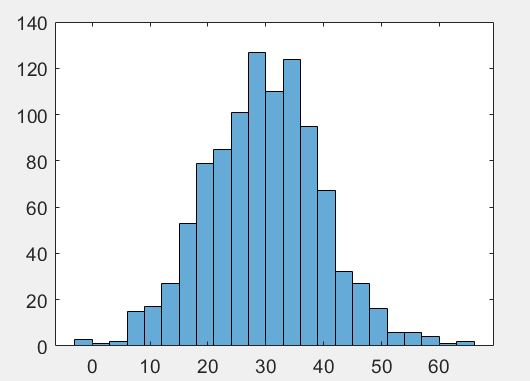
\includegraphics[scale=0.80]{day2_seg1_prob/histogram.jpg}
\end{center}
\end{footnotesize}
\end{frame}

\begin{frame}
  \onslide<1->{
	\frametitle{Empirical Statistics} 
	\framesubtitle{Sample Stats with MATLAB}
}
\begin{footnotesize}
True $\mu,\sigma$: mu=30;sigma=10;\\
10,000 samples: X=mu+sigma*\text{randn}(10000,1);\\
$\samplemean{X}=30.0563$ and $\samplevar{X}=97.3913$ (sample standard deviation $s_X=9.8687$)\\
\begin{center}
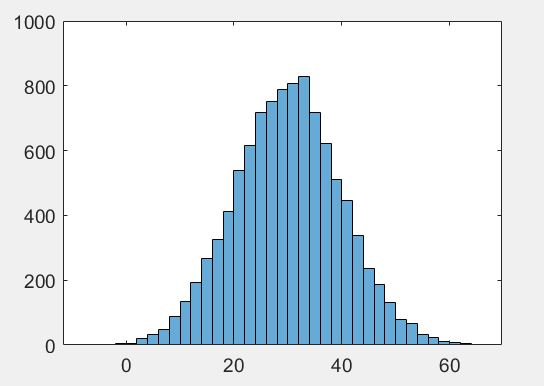
\includegraphics[scale=0.80]{day2_seg1_prob/histogram10000.jpg}
\end{center}
\end{footnotesize}
\end{frame}

\begin{frame}
  \onslide<1->{
	\frametitle{Empirical Statistics} 
	\framesubtitle{Sample Stats with MATLAB}
}
\begin{footnotesize}
True $\mu,\sigma$: mu=30;sigma=10;\\
10,000 samples: X=mu+sigma*\text{randn}(10000,1);\\
$\samplemean{X}=30.0563$ and $\samplevar{X}=97.3913$ (sample standard deviation $s_X=9.8687$)\\
\begin{center}
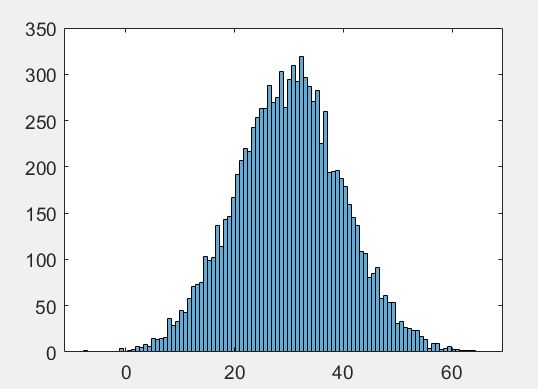
\includegraphics[scale=0.80]{day2_seg1_prob/histogram10000more_bins.jpg}
\end{center}
\end{footnotesize}
\end{frame}

\begin{frame}
  \onslide<1->{
	\frametitle{Empirical Statistics} 
	\framesubtitle{Sample Stats with MATLAB}
}
\begin{footnotesize}
True $\mu,\sigma$: mu=30;sigma=10;\\
10,000 samples: X=mu+sigma*randn(10000,1);\\
$\samplemean{X}=30.0563$ and $\samplevar{X}=97.3913$ (sample standard deviation $s_X=9.8687$)\\
$\;\;\;$\\
Define new random variable $Y$ to be linearly dependent on $X$ plus 
some random Gaussian noise:Y=3*X+2+randn(10000,1);\\
$\;\;\;$\\
MATLAB's corrcoef functions says (rightly) that $X$ and $Y$ are highly correlated: $r_{XY}=0.9994$
\end{footnotesize}
\end{frame}

% day1_seg4_prob/exercises.tex
\begin{frame}
  \onslide<1->{
	\frametitle{Probability and Statistics} 
	\framesubtitle{Exercises}
}
\begin{itemize}
  \onslide<2->{
 \item Show that $A\subseteq B\Rightarrow P(A)\leq P(B)$.\\
 (Hint: Use $B=A\cup (B\setminus A)$ and the fact that measures are additive.)
}
  \onslide<3->{
 \item Show that $P(A\cup B)=P(A)+P(B)-P(A\cap B)$
}
  \onslide<4->{
 \item Let $F$ be the distribution of a random variable $X$
 and suppose that $a\leq b$ are real numbers.  Show
 that $P(x\in [a,b))=F(b)-F(a)$.
}
\end{itemize}
\end{frame}
\begin{frame}
  \onslide<1->{
	\frametitle{Probabillity and Statistics} 
	\framesubtitle{Exercises}
}
\begin{itemize}
  \onslide<2->{
 \item Prove the following:  If two events $A$ and $B$ are
 independent, then the events $A$ and $B'$ are also independent.
}
  \onslide<3->{
 \item Show that for any distribution function $F$ of a random variable $X$,
  $P(X>a)=\lim_{x\downarrow a} F(x)$.
}
\end{itemize}
\end{frame}

\begin{frame}
  \onslide<1->{
	\frametitle{Statistics} 
	\framesubtitle{Exercises}
}
\begin{itemize}
  \onslide<2->{
 \item Let $\Omega$ be any sample space and $A\subseteq \Omega$.
  Let $X(\omega)=\chi_A(\omega)$.  Recall that
 $\chi_A(\omega)=
  \begin{cases}
    1 & \text{if } \omega\in A, \\
    0 & \text{otherwise}.
  \end{cases}$ \\
 Prove that
 $F(x)=
  \begin{cases}
    0   & \text{if } x<0, \\
    1-P(A) & \text{if } 0\leq x<1, \\
    1   &  \text{if } x\geq 1.
  \end{cases}$
}
\end{itemize}
\end{frame}

\begin{frame}
  \onslide<1->{
	\frametitle{Probability and Statistics} 
	\framesubtitle{Exercises}
}
\begin{itemize}
  \onslide<2->{
 \item A gyro manufacturer produces defective gyros with
 probability $p$, where $0<p<1$.  After a lot of $n$ independent
 gyros have been produced, they are
 examined.  Let $X$ denote the number of defective gyros in the
 lot.  What is the probability mass function of this discrete
 distribution?
}
\end{itemize}
\end{frame}



% day2_seg1_ranproc1/ranproc_main.tex
\begin{frame}
  \onslide<1->{
	\frametitle{Random Processes} 
	\framesubtitle{Topics}
}
\begin{itemize}
  \onslide<2->{
 \item Two Dimensions:  Ensemble vs. Time
}
  \onslide<3->{
 \item Stationary and Ergodic
}
  \onslide<4->{
 \item Correlation and Covariance
}
  \onslide<5->{
 \item Power Spectral Density
}
\end{itemize}
\end{frame}
% day2_seg1_ranproc1/twodim.tex


\begin{frame}
  \onslide<1->{
	\frametitle{Random Processes} 
	\framesubtitle{Two Dimensions:  Ensemble vs. Time}
}
\begin{itemize}
  \onslide<2->{
 \item Two equivalent ways to define a random process:  
 One way views a random process as a time function whose value at each 
 instant of time is a random variable.
}
  \onslide<3->{
 \item The other defines a random process as a function of two variables: 
 the outcomes $\omega\in\Omega$ and time $t$.  
}
  \onslide<4->{
 \item Outcomes $\omega$ belong to sample space $\Omega$ while times $t$ are represented as real numbers, 
 often non-negative.
}
\end{itemize}
\end{frame}

\begin{frame}
  \onslide<1->{
	\frametitle{Random Processes} 
	\framesubtitle{Two Dimensions:  Ensemble vs. Time}
}
\begin{itemize}
  \onslide<2->{
 \item At each fixed $t$, the random process $X(\cdot,t)$, or simply $X(t)$ is simply a random variable, 
 i.e., a function of the other variable $\omega$ alone
}
  \onslide<3->{
 \item For a fixed $\omega$, we have an ordinary time function of $t$.
}
\end{itemize}
\end{frame}


\begin{frame}
  \onslide<1->{
	\frametitle{Random Processes} 
	\framesubtitle{Definitions}
}
\begin{itemize}
  \onslide<2->{
 \item A \textit{\textbf{Random Process}} (also called a \textit{\textbf{stochastic process}}) is a
 function $X:[0,T]\rightarrow RV(\Omega)$, where $[0,T]$ is a
 closed interval of the real line.
}
  \onslide<3->{
 \item We think of variables $t\in [0,T]$ as time.
}
  \onslide<4->{
 \item The image of $t\in [0,T]$ under $X$ is a random variable:
 \[X(t):\Omega\rightarrow \Real\].
}
 \onslide<5->{
   \item The random variables $X(s)$ and $X(t)$ are not necessarily correlated in any way (when $x\neq t$)
 }
\end{itemize}
\end{frame}

\begin{frame}
  \onslide<1->{
	\frametitle{Random Processes} 
	\framesubtitle{Curves in Hilbert Space}
}
\begin{itemize}
  \onslide<2->{
 \item Thus a random process can be viewed as a function whose values are
 themselves functions
}
  \onslide<3->{
 \item We could also think of $X$ as a two-variable function from the Cartesian product 
 $[0,T]\times \Omega$ into the reals:
 \[X(t,\omega)\in \Real\]
}
\end{itemize}
\end{frame}

\begin{frame}
  \onslide<1->{
	\frametitle{Random Processes} 
	\framesubtitle{}
}
\begin{itemize}
  \onslide<2->{
 \item These two perspectives are interchangeable and we shall use
 both.
}
  \onslide<3->{
 \item We use all of the following notation for a random process 
\[X_t\]
\[X_t(\omega)\]
\[X(t)\]
\[X(t,\omega)\] 
}
\end{itemize}
\end{frame}


\begin{frame}
  \onslide<1->{
	\frametitle{Random Processes} 
	\framesubtitle{}
}
\begin{itemize}
  \onslide<2->{
 \item If you fix $\omega$ and let $t$ vary you get a \textit{\textbf{sample
 trajectory}}.
}
  \onslide<3->{
 \item In this way, you can think of $X$ as an ensemble of sample
 trajectories.
}
  \onslide<4->{
 \item Therefore, we will talk about both sample trajectory
 properties (continuity, differentiability, etc.) and ensemble
  properties (statistical).
}
\end{itemize}
\end{frame}

\begin{frame}
  \onslide<1->{
	\frametitle{Random Processes} 
	\framesubtitle{Random Process as Ensemble of Trajectories}
}
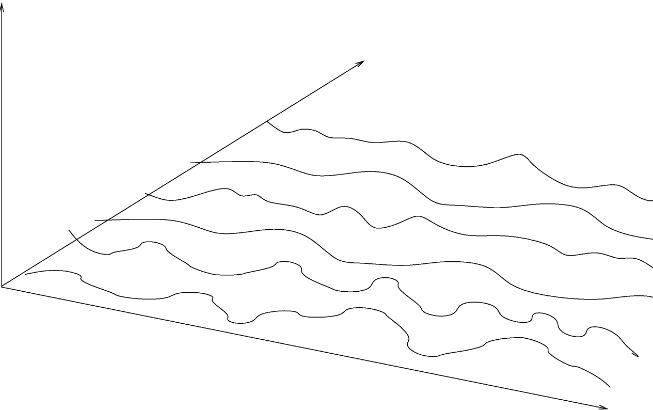
\includegraphics[scale=0.8]{day2_seg1_ranproc1/ensemble.jpg}
\end{frame}

\begin{frame}
  \onslide<1->{
	\frametitle{Random Processes} 
	\framesubtitle{Examples of Discrete Processes: Sampling with Replacement}
}
\begin{itemize}
  \onslide<2->{
			\item A card player shuffles a deck of cards and then picks a card at random.  
}
  \onslide<3->{
			\item He enters the value of the card (1 for an ace through 13 for a king) in an Excel spreadsheet column.  
}
  \onslide<4->{
			\item He then replaces the card and repeats the process over and over again.  
}
  \onslide<5->{
			\item After 10 such experiments, he begins anew with a new Excel column.  Each column represents a new sample trajectory. 
}
\end{itemize}
\end{frame}


\begin{frame}
  \onslide<1->{
	\frametitle{Random Processes} 
	\framesubtitle{Examples of Discrete Processes: MATLAB / Simulink Band-Limited White Noise}
}
\begin{itemize}
  \onslide<2->{
			\item A single source block (band-limited white noise) and a single sink (the scope).
}
  \onslide<3->{
			\item Each time the simulation is run, a new sample trajectory is generated.
}
  \onslide<4->{
			\item Note that this discrete process is created by supposedly sampling a continuous process.    
}
\end{itemize}
\end{frame}


\begin{frame}
  \onslide<1->{
	\frametitle{Random Processes} 
	\framesubtitle{Examples of Discrete Processes: MATLAB / Simulink Band-Limited White Noise}
}
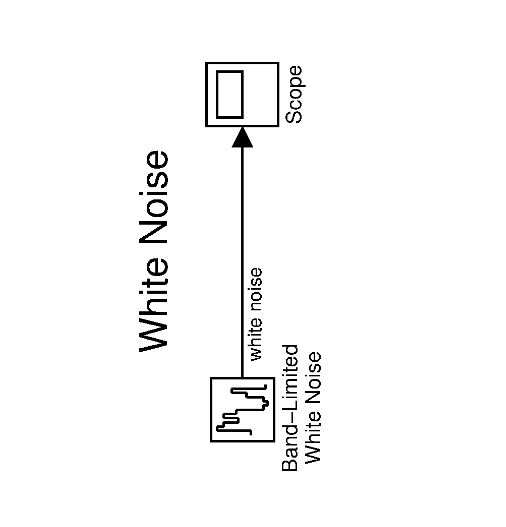
\includegraphics[angle=-90]{day2_seg1_ranproc1/white_noise.jpg}
\end{frame}


\begin{frame}
  \onslide<1->{
	\frametitle{Random Processes} 
	\framesubtitle{Examples:  MATLAB / Simunlink Random Constant}
}
\begin{itemize}
  \onslide<2->{
			\item A single source block (constant block with value generated by random number 
			generator) and a single sink (the scope).
}
  \onslide<3->{
			\item Each time the simulation is run, a new sample trajectory is generated.
}
  \onslide<4->{
			\item Note that this is a continuous process.  
}
\end{itemize}
\end{frame}

\begin{frame}
  \onslide<1->{
	\frametitle{Random Processes} 
	\framesubtitle{Examples:  MATLAB / Simunlink Random Constant}
}
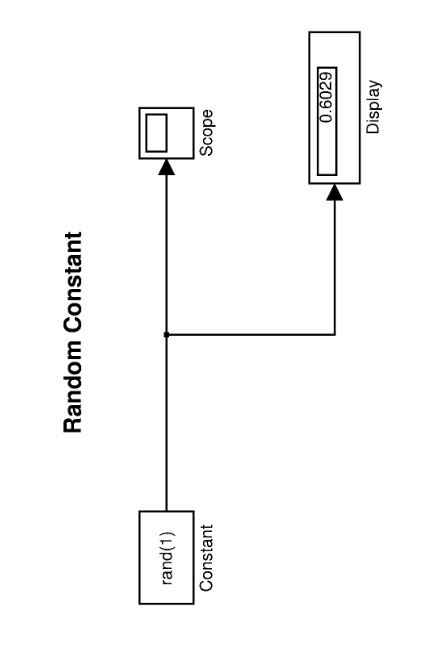
\includegraphics[angle=-90, scale=0.80]{day2_seg1_ranproc1/rand_const1.jpg}
\end{frame}


\begin{frame}
  \onslide<1->{
	\frametitle{Random Processes} 
	\framesubtitle{Examples:  MATLAB / Simunlink Random Constant}
}
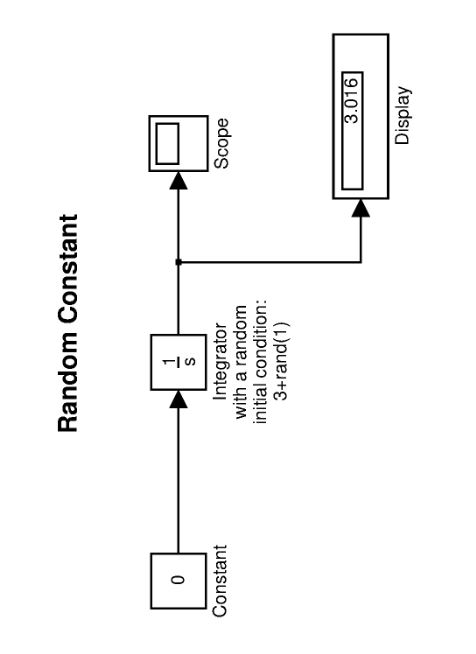
\includegraphics[angle=-90]{day2_seg1_ranproc1/rand_const2.jpg}
\end{frame}

\begin{frame}
  \onslide<1->{
	\frametitle{Random Processes} 
	\framesubtitle{MATLAB / Simulink Sine Wave with Random Phase}
}
\begin{itemize}
  \onslide<2->{
			\item A single source block (sine wave with random phase) and a single sink (the scope)
}
  \onslide<3->{
			\item Each time the simulation is run, a new sample trajectory is generated but 
			each time with a different value for the phase
}
  \onslide<4->{
			\item Note that this is a continuous process  
}
\end{itemize}
\end{frame}


\begin{frame}
  \onslide<1->{
	\frametitle{Random Processes} 
	\framesubtitle{MATLAB / Simulink Sine Wave with Random Phase}
}
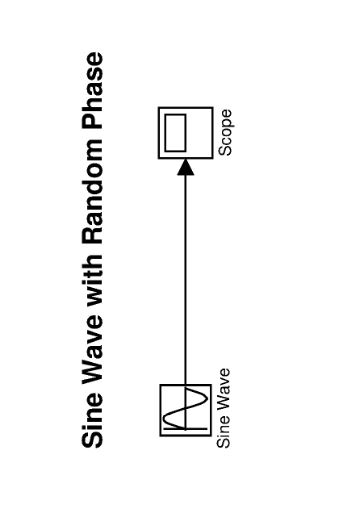
\includegraphics[angle=-90]{day2_seg1_ranproc1/sine_rand_phase.jpg}
\end{frame}

% day2_seg1_ranproc1/stationary.tex
\begin{frame}
  \onslide<1->{
	\frametitle{Random Processes} 
	\framesubtitle{Stationary Random Processes}
}
\begin{itemize}
  \onslide<2->{
 \item A process $X$ is called \textit{\textbf{strongly stationary}} if for
 any finite set of times $\set{t_1,\ldots,t_n}$ and any $\tau>0$
 the two sets of random variables $\set{X(t_1),\ldots,X(t_n)}$ and
$\set{X(t_1+\tau),\ldots,X(t_n+\tau)}$ have identical probability
distributions.
}
  \onslide<3->{
 \item $X$ is called \textit{\textbf{weakly stationary}} if
 \[ \expect{X(s)}=\expect{X(t)}\]
 and
 \[ \expect{X(s)X(t)}=\expect{X(s+\tau)X(t+\tau)}\]
 for all appropriate $\tau>0$ and all times $s,t$.
}
\end{itemize}
\end{frame}

% day2_seg1_ranproc1/corrcov.tex
\begin{frame}
  \onslide<1->{
	\frametitle{Random Processes} 
	\framesubtitle{Correlation and Covariance}
}
\begin{itemize}
  \onslide<2->{
 \item Since at each $t$ $X(t)$ is a random variable in its own right, it makes sense to talk about the correlation of two such random variables $X(t)$ and $X(s)$.
}
  \onslide<3->{
 \item Since both random variables come from the same underlying process, we refer to this as autocorrelation.
}
  \onslide<4->{
 \item Similarly, autocovariance involves first centering the process about its mean process $\mu_t$.
}
\end{itemize}
\end{frame}

\begin{frame}
  \onslide<1->{
	\frametitle{Random Processes} 
	\framesubtitle{Correlation and Covariance}
}
\begin{itemize}
  \onslide<2->{
 \item The function $\expect{X(t)X(t+\tau)}$ is called the \textit{\textbf{autocorrelation
 function}} of $X$ and for a weakly stationary process $X$, and it is denoted by
 $R_{XX}(\tau)$, since it is a function of $\tau$ alone.
}
  \onslide<3->{
 \item The \textit{\textbf{autocovariance}} function for a weakly stationary process is formed
 by subtracting out the means:
 $C_{XX}(\tau)=\expect{(X(t)-\mu_t)(X(t+\tau)-\mu_{t+\tau})}$.
}
  \onslide<4->{
 \item Cross correlation and cross covariance between two different random processes $X$
 and $Y$ are defined in the obvious way.
}
 \onslide<5->{
 \item Note that these are difference than the sample cross correlation and sample cross covariance that 
 we deal with in empirical work
}
\end{itemize}
\end{frame}

\begin{frame}
  \onslide<1->{
	\frametitle{Random Processes} 
	\framesubtitle{Examples of Autocorrelation Functions}
}
\begin{itemize}
  \onslide<2->{
\item Consider the random process $X(t,\omega)=A(\omega)\sin(2\pi f t+\theta)$ in which $A:\Omega\rightarrow \Real$ is a normally distributed random variable with variance $\sigma^2$.
}
  \onslide<3->{
\item The autocorrelation function $R_{XX}(s,t)$ is therefore
\begin{align*}
\expect{X(t,\omega)X(s,\omega)}&=\expect{A(\omega)\sin(2\pi f t+\theta)A(\omega)\sin(2\pi f s+\theta)}\\
&=\expect{A(\omega)^2}\sin(2\pi f t+\theta)\sin(2\pi f s+\theta)\\
&=\sigma^2\sin(2\pi f t+\theta)\sin(2\pi f s+\theta)
\end{align*}
}
\end{itemize}
\end{frame}
\begin{frame}
  \onslide<1->{
	\frametitle{Random Processes} 
	\framesubtitle{Examples of Autocorrelation Functions}
}
\begin{itemize}
  \onslide<2->{
\item Consider the white noise process $W(t)$.
}
  \onslide<3->{
\item Characteristic of white noise to be uncorrelated in time
}
  \onslide<4->{
\item Thus, $\expect{W(t)W(s}=0$ for every $s$ and $t$ such that $s\neq t$.
}
\end{itemize}
\end{frame}

\begin{frame}
  \onslide<1->{
	\frametitle{Random Processes} 
	\framesubtitle{Ergodic Processes}
}
\begin{itemize}
  \onslide<2->{
 \item We shall be concerned almost exclusively with weakly
 stationary processes that are also \textbf{ergodic}, meaning that ensemble
 averaging at any one time gives the same result as time averaging
 one sample trajectory.  Thus we may assume:
}
  \onslide<3->{
\begin{equation}\label{ergodic_mean}
  \mu_X=\limint X(t)dt
\end{equation}
}
  \onslide<4->{
\begin{equation}\label{ergodic_meansquare}
  \psi_X^2 = \limint X^2(t)dt
\end{equation}
}
  \onslide<5->{
\begin{equation}\label{ergodic_autocorr}
  R_{XX}(\tau)=\limint X(t)X(t+\tau)dt
\end{equation}
}
\end{itemize}
\end{frame}

\begin{frame}
  \onslide<1->{
	\frametitle{Random Processes} 
	\framesubtitle{Ergodic Processes}
}
\begin{itemize}
  \onslide<2->{
 \item We haven't yet defined want we mean by such time integrals,
 however, so we have to hold off dealing with them.
}
  \onslide<3->{
 \item Once we have defined the mean square limit of
 Riemann-Stieltjes sums, then we'll know what these integrals
 really mean.
}
  \onslide<4->{
 \item Nevertheless, if we fix $\omega$ and consider only sample trajectories $X(t,\omega)$, then we can use ordinary integrals provided that the sample trajectories are well-enough behaved.
}
\end{itemize}
\end{frame}

\begin{frame}
  \onslide<1->{
	\frametitle{Random Processes} 
	\framesubtitle{Ergodic Processes}
}
\begin{itemize}
  \onslide<2->{
 \item Well-behaved means that they are of bounded variation, i.e., they don't wiggle around too much.
}
  \onslide<3->{
 \item Unfortunately, this doesn't really work for the usual conception of white noise, because its sample trajectories are not of bounded variation.
}
  \onslide<4->{
 \item If we restrict our attention to band-limited white noise (like Matlab / Simulink does), then we can stick to the ordinary integrals we learned in calculus.
}
\end{itemize}
\end{frame}

% day2_seg1_ranproc1/psd.tex
\begin{frame}
  \onslide<1->{
	\frametitle{Random Processes} 
	\framesubtitle{Power Spectral Density}
}
\begin{itemize}
  \onslide<2->{
 \item The \textit{\textbf{power spectral density}} (PSD) function is the
 Fourier transform of the autocorrelation function:
\begin{equation}\label{psd}
  P_{XX}(\omega)=\infint R_{XX}(\tau)\exp(-j\omega\tau)d\tau
\end{equation}
where $j=\sqrt{-1}$ and $\omega$ is angular frequency in rad/sec (not an outcome of the sample space!).
}
  \onslide<3->{
 \item Units:  If $X$ is in volts(V), then
 $P_{XX}$ has units of $\text{V}^2/(2\pi \text{Hz})$ or $\text{V}^2\;\text{sec}/\text{rad}$, 
 due to $R_{XX}$ being a product of samples in volts and transform kernel
 being in 1/rad:
 $\exp(-j\omega\tau)=\frac{1}{\exp(j\omega\tau)}$.  $d\tau$ is in sec.
}
 \onslide<4->{
	\item Note: $2\pi\text{ rad/cycle }1\text{Hz}=2\pi\text{ rad/cycle }1\text{ cycle}/\text{sec}=2\pi\text{ rad/sec}$.
 }
\end{itemize}
\end{frame}
\begin{frame}
  \onslide<1->{
	\frametitle{Random Processes} 
	\framesubtitle{Power Spectral Density}
}
\begin{itemize}
  \onslide<2->{
 \item Sometimes the definition in equation \eqref{psd} is referred to as the autospectral
 density, since the autocorrelation function is involved
}
  \onslide<3->{
 \item The cross-spectral density function is defined in the same
 way, but with $R_{XY}$ substituted for $R_{XX}$
}
\end{itemize}
\end{frame}

\begin{frame}
  \onslide<1->{
	\frametitle{Random Processes} 
	\framesubtitle{Power Spectral Density}
}
\begin{itemize}
  \onslide<2->{
\item Another way to obtain power spectral density is through
 Fourier transform of the original process
}
 \onslide<3->{
\item Let's change our notation:  We've been using uppercase letters such as $X$ and $Y$ to
denote random variables and processes and we've been using $\omega$ to denote a
point of the sample space $\Omega$
}
  \onslide<4->{
\item Now we'll use lowercase letters like $x(t)$ and $y(t)$
to denote processes in the time domain but uppercase letters for
Fourier transforms in the frequency domain  
}
  \onslide<5->{
\item Also, lowercase $\omega$ will often stand for frequency in rad/sec
}
\end{itemize}
\end{frame}
\begin{frame}
  \onslide<1->{
	\frametitle{Random Processes} 
	\framesubtitle{Power Spectral Density}
}
\begin{itemize}
  \onslide<2->{
\item The finite Fourier transform of a random process $x(t)$ is
\[X(\omega,T)=\int_0^Tx(\tau)\exp(-j\omega\tau)d\tau\]
}
  \onslide<3->{
\item The PSD can be expressed as follows:
\begin{equation}\label{wiener_khinchin}
  P_{XY}(\omega) = \lim_{T\rightarrow \infty}\frac{1}{T}\expect{X^*(\omega,T)Y(\omega,T)}
\end{equation}
where $X(\omega,T)$ and $Y(\omega,T)$ are the finite Fourier
transforms of $x(t)$ and $y(t)$, respectively, and
$X^*(\omega,t)$ is the complex conjugate of $X(\omega,t)$. \\
$\omega$ is frequency in rad/sec.
}
  \onslide<4->{
\item Both Eq. \eqref{wiener_khinchin} and \eqref{psd} are referred to as the Wiener-Khinchin equation
}
\end{itemize}
\end{frame}


%% day2_seg1_ranproc1/exercises.tex
\begin{frame}
Exercises
 \begin{itemize}
 \item
 \item
 \item
\end{itemize}
\end{frame}


% day2_seg2_ranproc2/ranproc2_main.tex
\begin{frame}
  \onslide<1->{
	\frametitle{Random Processes} 
	\framesubtitle{Some Important Random Processes}
}
\begin{itemize}
  \onslide<2->{
 \item White Noise
}
  \onslide<3->{
 \item Random Walk
}
  \onslide<4->{
 \item Random Constant
}
  \onslide<5->{
 \item Random Ramp
}
  \onslide<6->{
 \item Second Order Processes:  Gaussian, and Gauss-Markov Processes
}
  \onslide<7->{
 \item State Space Augmentation
}
\end{itemize}
\end{frame}

% day2_seg2_ranproc2/white_noise.tex
\begin{frame}
  \onslide<1->{
	\frametitle{Some Important Random Processes} 
	\framesubtitle{White Noise}
}
\begin{itemize}
  \onslide<2->{
 \item White noise can be defined as a process whose
 autocorrelation function is a Dirac delta function:
\begin{equation}\label{dirac}
  \delta(\tau)=
  \begin{cases}
    \infty & \text{if }, \tau=0 \\
    0 & \text{otherwise}.
  \end{cases}
\end{equation}
}
  \onslide<3->{
 \item There's only one mathematical problem:  this is not a real function
}
  \onslide<4->{
 \item There's also a physical problem:  such a process would have
 infinite mean-squared value and hence infinite energy
}
\end{itemize}
\end{frame}
\begin{frame}
  \onslide<1->{
	\frametitle{Some Important Random Processes} 
	\framesubtitle{White Noise}
}
\begin{itemize}
  \onslide<2->{
 \item There is a way to properly define the Dirac delta as a linear functional (a distribution) rather than 
 a function, and to show that it retains all of its desired properties
  }
  \onslide<3->{
 \item However, we'll proceed as if this concept of white noise were well-defined and use the 
 delta function's integration properties to define some other processes such as random walk.
}
  \onslide<4->{
 \item Characteristic feature of white noise to be uncorrelated in time.  This is the intent of using the 
 Dirac delta functional as its defining autocorrelation function
}
\end{itemize}
\end{frame}
\begin{frame}
  \onslide<1->{
	\frametitle{Some Important Random Processes} 
	\framesubtitle{White Noise}
}
\begin{itemize}
  \onslide<2->{
 \item MATLAB / Simulink block for white noise makes it a bandlimited signal, so that the bandwidth is not 
 infinite as it otherwise would be for pure white noise
}
  \onslide<3->{
 \item Valid assumption as long as noise bandwidth is
 sufficiently greater than that of the system under consideration
 }
  \onslide<4->{
 \item In MATLAB you can simulate a discrete white noise sequence
 by drawing a random number at each time step from a normal distribution
}
  \onslide<5->{
 \item Bottom line:  Random sequence for white noise needs to have a correlation time much smaller than 
 the shortest time constant of the system
}
\end{itemize}
\end{frame}


% day2_seg2_ranproc2/rand_walk.tex
\begin{frame}
  \onslide<1->{
	\frametitle{Some Important Random Processes} 
	\framesubtitle{Random Walk}
}
\begin{itemize}
  \onslide<2->{
 \item In engineering applications, random walk is often considered as a discrete time process.
}
  \onslide<3->{
 \item Some authors (Gelb, for example) refer to continuous-time random walk as the
 solution of a differential equation driven by white noise:
 $\dot{x}=w$.
}
  \onslide<4->{
 \item However, that would require $w$ to be integrable which it is not, because it is not of bounded variation.  
 Alternatively, it would require the Wiener-Levy process to be differentiable, which it is not
}
  \onslide<5->{
 \item So we'll stick to the bandlimited or the discrete case: $x(k+1)=x(k) + w(k)$,
 where the $w(k)$ are normally distributed and statistically uncorrelated at distinct sample times
}
\end{itemize}
\end{frame}

\begin{frame}
  \onslide<1->{
	\frametitle{Some Important Random Processes} 
	\framesubtitle{Random Walk:  Bandlimited White Noise is Integrable}
}
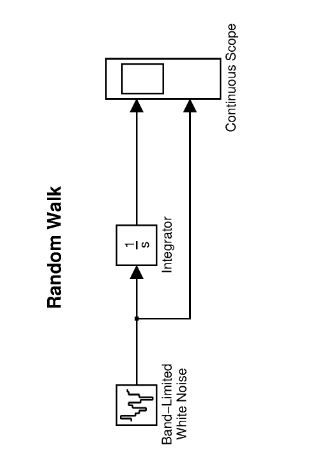
\includegraphics[angle=-90, scale=0.80]{day2_seg2_ranproc2/rand_walk.jpg}
\end{frame}

\begin{frame}
  \onslide<1->{
	\frametitle{Some Important Random Processes} 
	\framesubtitle{Discrete Random Walk}
}
\begin{itemize}
  \onslide<2->{
\item  $x(k)=x(k-1)+w(k)$, where $w(k)$ is a white sequence 
}
  \onslide<3->{
\item  Another way of looking at this is to say that the difference sequence is white:  $x(k)-x(k-1)=w(k)$ 
}
  \onslide<4->{
\item  In MATLAB you can use the diff function to create the difference sequence from a give sequence. Note that 
it would have 1 less element than the original sequence:\\
x=rand(1,5); dx=diff(x);\\
x =    [ 1,     0,     2,    -1,     4]\\
dx =  [-1,     2,    -3,     5] 
}
\end{itemize}
\end{frame}

\begin{frame}
  \onslide<1->{
	\frametitle{Some Important Random Processes} 
	\framesubtitle{Discrete Random Walk:  Raytheon Stock Price (4000 daily samples)}
}
\begin{center}
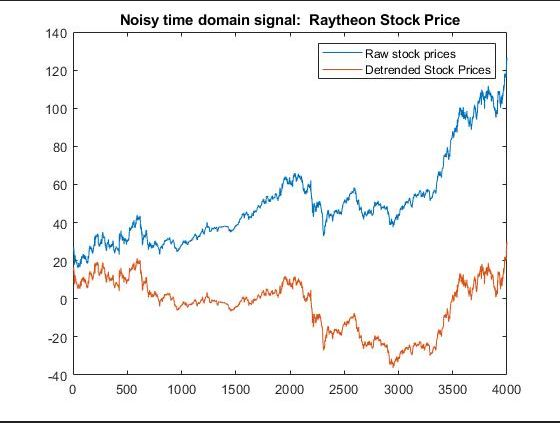
\includegraphics[scale=0.50]{day2_seg2_ranproc2/rtn_stock_prices.jpg}
\end{center}
\end{frame}
 
\begin{frame}
  \onslide<1->{
	\frametitle{Some Important Random Processes} 
	\framesubtitle{Discrete Random Walk:  Raytheon Stock Price Power Spectal Density}
}
\begin{center}
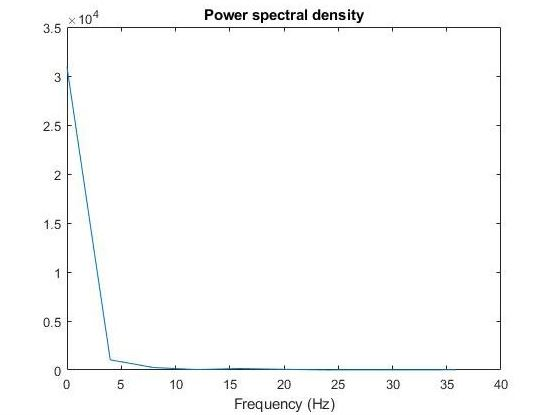
\includegraphics[scale=0.50]{day2_seg2_ranproc2/rtn_randwalk.jpg}
\end{center}
\end{frame}

\begin{frame}
  \onslide<1->{
	\frametitle{Some Important Random Processes} 
	\framesubtitle{Discrete Random Walk:  Detrened Difference of Raytheon Stock Price}
}
Let's see if the difference sequence of detrended stock prices looks like white noise:
\begin{center}
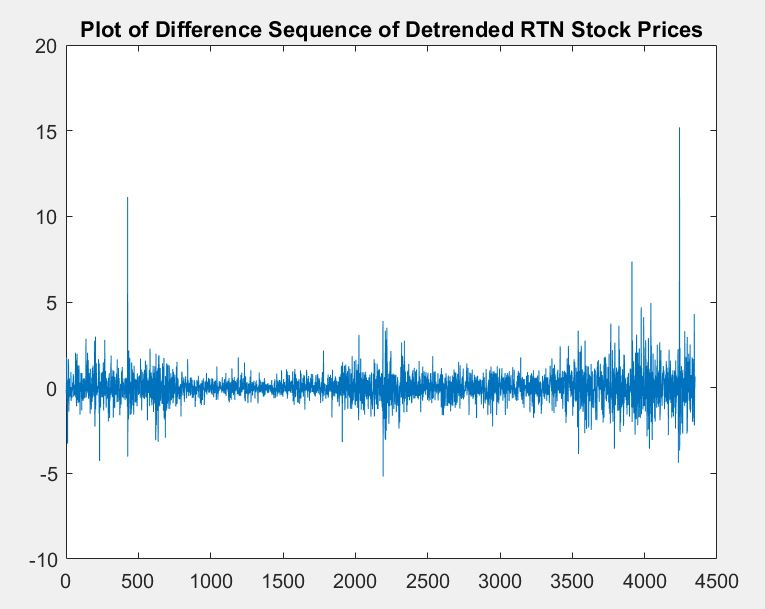
\includegraphics[scale=0.50]{day2_seg2_ranproc2/rtn_stock_prices_diff_detrended.jpg}
\end{center}
\end{frame}

% day2_seg2_ranproc2/rand_ramp.tex
\begin{frame}
  \onslide<1->{
	\frametitle{Some Important Random Processes} 
	\framesubtitle{Random Constant and Random Ramp}
}
\begin{itemize}
  \onslide<2->{
 \item A random constant process $x$ such that the sample trajectories are constant with respect to time\\
\begin{footnotesize} But the constant value is different for each sample trajectory in the ensemble\\
$x(\omega_1,t)\neq x(\omega_2,t)$, for $\omega_1\neq \omega_2$
\end{footnotesize}
}
  \onslide<3->{
 \item A random ramp requires two state variables: a random constant (y-intercept or bias) and the integral of a
 random constant (yields random slope)
}
  \onslide<4->{
 \item In principle,
 however, this constant value could vary with $\omega$, i.e., across the
 ensemble, thus making the process non-Ergodic.
}
  \onslide<5->{
 \item Random constants are very useful in many applications to model biases that vary from
 turn-on to turn-on
}
\end{itemize}
\end{frame}
\begin{frame}
  \onslide<1->{
	\frametitle{Some Important Random Processes} 
	\framesubtitle{Random Constant and Random Ramp}
}
\begin{itemize}
  \onslide<2->{
 \item See Matlab Simulink demos:  rand\_const.mdl and
 rand\_ramp.mdl
}
  \onslide<3->{
 \item In modeling gyro biases, a combination of a random constant
 (bias stability) and random walk (bias drift) is common.
}
  \onslide<4->{
 \item Gyro scale factors are modeled similarly.
}
  \onslide<5->{
 \item Deterministic biases and scale factors are also part of the model, but these generally are calibrated out.
}
\end{itemize}
\end{frame}

% day2_seg2_ranproc2/markov_proc.tex
\begin{frame}
  \onslide<1->{
	\frametitle{Some Important Random Processes} 
	\framesubtitle{Second Order Processes}
}
\begin{itemize}
  \onslide<2->{
 \item We will generally restrict our attention to \textit{\textbf{second-order processes}}, i.e., those such that
 $X(t)\in L^2(\Omega)$.
 \item Recall what this means:
 \[\expect{X^2(t)}<\infty\]
}
  \onslide<3->{
 \item This allows us to use Hilbert space techniques because, for
 every $s,t\in[0,T]$, $\expect{X(s)Y(t)}$ is an inner
 product.  Inner products, norms and metrics allow us to do
 calculus and geometry (orthogonal projection).
}
\end{itemize}
\end{frame}

\begin{frame}
  \onslide<1->{
	\frametitle{Some Important Random Processes} 
	\framesubtitle{Orthogonal Projection}
}
\begin{center}
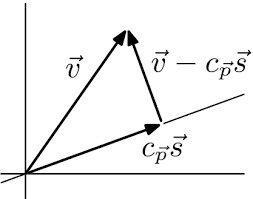
\includegraphics[scale=0.6]{graphics/orthoproj.png}
\end{center}
\end{frame}


\begin{frame}
  \onslide<1->{
	\frametitle{Some Important Random Processes} 
	\framesubtitle{Gaussian Processes}
}
\begin{itemize}
  \onslide<2->{
 \item An important class of second-order processes are the
 Gaussian processes.
}
  \onslide<3->{
\item Let $X:[0,T]\rightarrow L^2(\Omega)$ be a second-order
 process.  $X$ is said to be \textit{\textbf{Gaussian}} if for every finite set of times $\set{t_1,\ldots,t_n}$
 the vector of random variables $(X(t_1),\ldots,X(t_n))$ has a
 multivariate normal distribution.
}
  \onslide<4->{
  \item To fully appreciate what this means, we need to explain
 what a multivariate normal distribution is.
}
\end{itemize}
\end{frame}

\begin{frame}
  \onslide<1->{
	\frametitle{Some Important Random Processes} 
	\framesubtitle{Gaussian Processes}
}
\begin{itemize}
  \onslide<2->{
 \item A function $Q_C:\Real^n\rightarrow \Real$ of the form
 \[Q_C(x)=x\trans C x\]
 where $x\in\Real^n$ is a column vector and $C$ is a real symmetric
 matrix., is called a \textit{\textbf{quadratic form}} associated with $C$. (I.e., $C=(c_{ij})$ and $c_{ij}=c_{ji}$).
}
  \onslide<3->{
 \item We will further assume that $C$ is positive definite, which
 means that $Q_{C}(x)>0$ for every non-zero vector $x$.
}
\end{itemize}
\end{frame}

\begin{frame}
  \onslide<1->{
	\frametitle{Some Important Random Processes} 
	\framesubtitle{Gaussian Processes}
}
\begin{itemize}
  \onslide<2->{
 \item Then $X_1,\ldots,X_n$ are said to have a \textit{\textbf{multivariate normal distribution}}
 if their joint p.d.f. is of the form
\begin{equation}\label{gaussvec}
  f(x_1,\ldots,x_n)=\gvpdf
\end{equation}
for a real, positive definite symmetric matrix $C$ and
$\mu=(\mu_1,\ldots,\mu_n)$.
}
  \onslide<3->{
 \item $C$ is called the \textit{\textbf{covariance matrix}} and $\mu$ is called the
 \textit{\textbf{mean}} vector.
}
\end{itemize}
\end{frame}

\begin{frame}
  \onslide<1->{
	\frametitle{Some Important Random Processes} 
	\framesubtitle{Gaussian Processes}
}
\begin{itemize}
  \onslide<2->{
 \item In terms of quadratic forms, this is
 \[f(x_1,\ldots,x_n)= \sqrt{\frac{\det(C^{-1})}{(2\pi)^n }}
  \exp\left[ -\frac{1}{2}Q_{C^{-1}}(x-\mu) \right]\]
}
  \onslide<3->{
\item $C^{-1}$ is sometimes called the information matrix,
 because its inverse, the covariance matrix, often expresses the
 uncertainty (or lack of information) associated with the random
 variables.
}
\end{itemize}
\end{frame}

\begin{frame}
  \onslide<1->{
	\frametitle{Some Important Random Processes} 
	\framesubtitle{Gaussian Processes}
}
\begin{itemize}
  \onslide<2->{
\item Thus a Gaussian process is a random process for which the
 joint distribution of every finite collection of range random
 variables is a Gaussian distribution.
}
  \onslide<3->{
  \item The Gaussian process is important in connection with the
 kinds of noise that drive the dynamic systems we are interested
 in.
}
  \onslide<4->{
 \item The linear Kalman filter is optimal only under assumptions
 that the process noise and the measurement noise are Gaussian.
}
\end{itemize}
\end{frame}

\begin{frame}
  \onslide<1->{
	\frametitle{Some Important Random Processes} 
	\framesubtitle{Gauss-Markov Processes}
}
\begin{itemize}
  \onslide<2->{
 \item A Gauss-Markov process is for which the autocorrelation
 function has an exponential form:
\begin{equation}\label{gauss-markov}
  R_{XX}(\tau) = \sigma^2\exp(-\beta\abs{\tau})
\end{equation}
}
  \onslide<3->{
\item As a continuous-time dynamic system, this would correspond to passing white
 noise through first-order feedback system:
 \[\dot{x}=-\beta x+w\]
 \item See Matlab Simulink file gauss\_markov.mdl
}
\end{itemize}
\end{frame}

\begin{frame}
  \onslide<1->{
	\frametitle{Some Important Random Processes} 
	\framesubtitle{Gauss-Markov Processes}
}
\begin{itemize}
  \onslide<2->{
\item Discrete version of a Gauss-Markov process:
\[
x(k+1)=\exp\left(-\beta \Delta t\right)x(k) + w(k)
\]
where $\Delta t = t_{k+1}-t_k$ and is assumed to be the same regardless of $k$, and $w(k)$ is a white noise sequence
}
\end{itemize}
\end{frame}
\begin{frame}
  \onslide<1->{
	\frametitle{Some Important Random Processes} 
	\framesubtitle{Gauss-Markov Processes:  Simulink Model}
}
\begin{center}
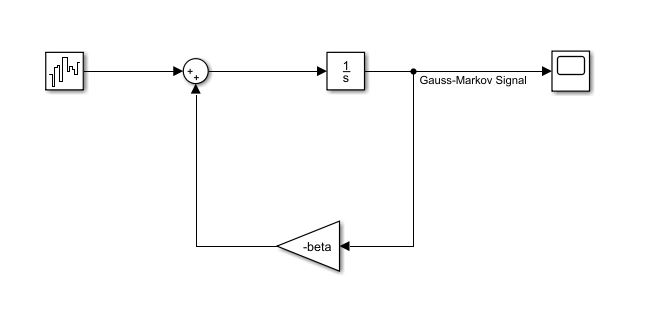
\includegraphics[scale=0.60]{day2_seg2_ranproc2/gauss_markov.jpg}
\end{center}
\end{frame}
\begin{frame}
  \onslide<1->{
	\frametitle{Some Important Random Processes} 
	\framesubtitle{Gauss-Markov Processes:  Output of Simulink Model}
}
\begin{center}
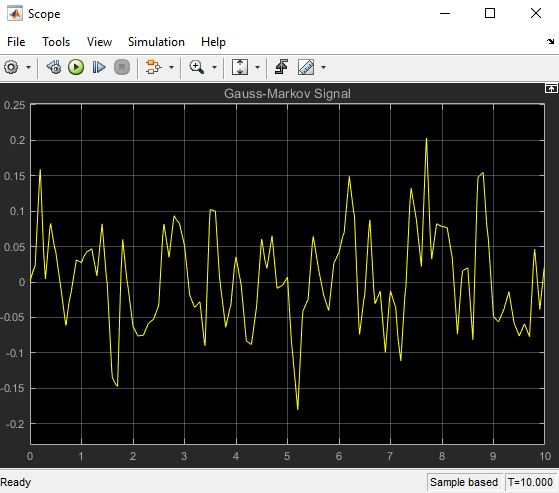
\includegraphics[scale=0.50]{day2_seg2_ranproc2/gauss_markov_scope.jpg}
\end{center}
\end{frame}

% day2_seg2_ranproc2/state_space_aug.tex
\begin{frame}
  \onslide<1->{
	\frametitle{State Space Augmentation} 
	\framesubtitle{Motivation}
}
\begin{itemize}
  \onslide<2->{
 \item Kalman filter theory assumes the only remaining forcing function is white process noise
}
  \onslide<3->{
 \item The most frequently used models can all be understood as differential equations (or difference equations) 
 driven by white noise
}
  \onslide<4->{
 \item If assumption of the only forcing function being white is not satisfied due to presence of colored noise, 
 then the colored noise can be whitened
}
  \onslide<5->{
 \item Otherwise, new states need to be added:  this is called state vector or state space \textbf{augmentation}
}
  \onslide<6->{
 \item We'll see an example of state space augmentation later when we discuss filter maintenance
}
\end{itemize}
\end{frame}

\begin{frame}
  \onslide<1->{
	\frametitle{State Space Augmentation} 
	\framesubtitle{General Example:  Augmenting a 2-State Model}
}
\begin{itemize}
  \onslide<2->{
\item Given 2-state model:  
\[
\begin{bmatrix}
\dot{x}_1\\
\dot{x}_2

\end{bmatrix} =
\begin{bmatrix}
a_{11} & a_{12}\\
a_{21} & a_{22}
\end{bmatrix}
\begin{bmatrix}
x_1\\
x_2
\end{bmatrix}+
\begin{bmatrix}
w_1\\
w_2
\end{bmatrix}
\]  
}
  \onslide<3->{
\item  Suppose the "noise" is not actually white;  perhaps there is some long-term drift as exhibited by random walk
}
  \onslide<4->{
\item   This means that $\dot{w}_i=\epsilon_i$, where $\epsilon_i$ is white
}
  \onslide<5->{
\item We augment with new states $x_3=w_1,x_4=w_2$ as follows: 
\[
\begin{bmatrix}
\dot{x}_1\\
\dot{x}_2\\
\dot{x}_3\\
\dot{x}_4

\end{bmatrix} =
\begin{bmatrix}
a_{11} & a_{12} & 1 & 0\\
a_{21} & a_{22} & 0 & 1\\
0 & 0 & 0 & 0\\
0 & 0 & 0 & 0
\end{bmatrix}
\begin{bmatrix}
x_1\\
x_2\\
x_3\\
x_4
\end{bmatrix}+
\begin{bmatrix}
0 & 0 & 0 & 0\\
0 & 0 & 0 & 0\\
0 & 0 & 1 & 0\\
0 & 0 & 0 & 1

\end{bmatrix}
\begin{bmatrix}
0\\
0\\
\epsilon_1\\
\epsilon_2
\end{bmatrix}
\]  
}
\end{itemize}
\end{frame}
\begin{frame}
  \onslide<1->{
	\frametitle{State Space Augmentation} 
	\framesubtitle{}
}
\begin{itemize}
  \onslide<2->{
\item   If original measurement was, say,
\[
\begin{bmatrix}
z_1\\
z_2
\end{bmatrix}=
\begin{bmatrix}
1 & 0\\
0 & 1
\end{bmatrix}
\begin{bmatrix}
x_1\\
x_2
\end{bmatrix}+
\begin{bmatrix}
v_1\\
v_2
\end{bmatrix}
\]
}
  \onslide<3->{
\item  It now becomes, after augmentation: 
\[
\begin{bmatrix}
z_1\\
z_2
\end{bmatrix}=
\begin{bmatrix}
1 & 0 & 0 & 0\\
0 & 1 & 0 & 0
\end{bmatrix}
\begin{bmatrix}
x_1\\
x_2\\
x_3\\
x_4
\end{bmatrix}+
\begin{bmatrix}
v_1\\
v_2
\end{bmatrix}
\]
}
\end{itemize}
\end{frame}
\begin{frame}
  \onslide<1->{
	\frametitle{State Space Augmentation} 
	\framesubtitle{How can you tell when to augment your state vector?}
}
\begin{itemize}
  \onslide<2->{
\item To determine if state vector augmentation is needed, look at the pre-fit residual sequence:  $\nu(k)=\innovation{k}$  
}
  \onslide<3->{
\item Examine its autocorelation function $R_{\nu\nu}$ (or autospectal density)  
}
  \onslide<4->{
\item Determine the correlation time constant and augment the state vector with a Gauss-Markov process with the appropriate
time constant in the feedback gain 
}
  \onslide<5->{
\item Alternatively, you can examine the autospectal density graph and eyeball a correlation constant (See Grewal handouts.)  
}
\end{itemize}
\end{frame}


% day2_seg2_ranproc2/exercises.tex
\begin{frame}
  \onslide<1->{
	\frametitle{Exercises} 
}
  \onslide<2->{
 1. Perform the following random walk experiment: \\
a. Create a graph with two axes marked off at integral (discrete) points.\\
b. Plot the first point at the origin.\\
c. Flip a coin.  If the result is heads, move one step to the right and plot a point 1 unit above the previous y value.  If the result is tails, move one step to the right and plot a point 1 unit below the previous y value.\\
d. Repeat step c ten times.\\
}
  \onslide<3->{
2.  What is your estimate for how the variance of this process grows with time?\\
}
  \onslide<4->{
3. As a class exercise, we'll compute the ensemble averages across the class results at each point.  Is this pocess ergodic?
}
\end{frame}


% day2_seg3_kalstats/kalstats_main.tex
\begin{frame}
  \onslide<1->{
	\frametitle{Kalman Statistics}
		\framesubtitle{Topics}
}
\begin{itemize}
  \onslide<2->{
 \item Covariance Matrices
}
  \onslide<3->{
 \item Process Noise Covariance Matrix $Q$
}
  \onslide<4->{
 \item Measurement Noise Covariance Matrix $R$
}
 \onslide<5->{
  \item Estimation Error Covariance Matrix $P$
 }
 \onslide<6->{
  \item Kalman Assumptions
 }
  \onslide<7->{
 \item The Static Estimation Problem:  Bayesian Derivation of the Kalman Gain
}
\end{itemize}
\end{frame}
% day2_seg3_kalstats/cov_mat.tex
\begin{frame}
  \onslide<1->{
	\frametitle{Covariance Matrices} 
	\framesubtitle{$Q,R,P$}
}
\begin{itemize}
  \onslide<2->{
 \item There are several covariance matrices associated with the Kalman filter: 
 $ \procnoisemat{k},\measnoisemat{k}, P(k)$
}
  \onslide<3->{
 \item In general, a covariance matrix is associated with a random vector $X$ as in the following definition:
\[C_X = \expect{XX\trans}\]
}
\end{itemize}
\end{frame}
\begin{frame}
  \onslide<1->{
	\frametitle{Covariance Matrices} 
	\framesubtitle{$Q,R,P$}
}
\begin{itemize}
  \onslide<2->{
 \item This is precisely how $\procnoisemat{k}$ and $\measnoisemat{k}$ are defined:
\[\procnoisemat{k}=\expect{w(k)w\trans(k)}\] and
\[\measnoisemat{k}=\expect{v(k)v\trans(k)}\]
}
  \onslide<3->{
\item $\covmat{k}{+}$, on the other hand is called the error covariance, because it is associated with $\esterr$
\[\covmatdef\]
where $\esterrdef$.
}
\end{itemize}
\end{frame}
\begin{frame}
  \onslide<1->{
	\frametitle{Covariance Matrices} 
	\framesubtitle{Positive Definite Symmetric Matrices}
}
\begin{itemize}
  \onslide<2->{
\item Covariance Matrices are \textbf{positive definite}: The quadratic form $x\trans C x>0$ for all nonzero vectors $x$  
}
  \onslide<3->{
\item We write $C>0$ for positive definite matrices  
}
  \onslide<4->{
\item $C>0$ iff all eigenvalues of $C$ are positive 
}
  \onslide<5->{
\item All diagonal elements of $C$ are positive if $C>0$  
}
  \onslide<6->{
\item If $C>0$ and $S$ non-singular (invertible), then $SCS\trans>0$ and $S\trans CS>0$
}
  \onslide<7->{
\item If $C>0$ then $C$ is non-singular and $C^{-1}>0$
}
\end{itemize}
\end{frame}

\begin{frame}
  \onslide<1->{
	\frametitle{Covariance Matrices} 
	\framesubtitle{Lower Triangular Cholesky Decomposition}
}
\begin{itemize}
  \onslide<2->{
\item  If $C>0$ then a lower triangular matrix $L$ can be found such that $C=LL\trans$ 
}
  \onslide<3->{
\item $L$ is called a \textbf{matrix square root} of $C$  
}
  \onslide<4->{
\item  Square root matrices are not unique;  $TL$ is also a square root of $C$ if $L$ is such and if $T$ is orthogonal $TT\trans=I$ 
}
  \onslide<5->{
\item We'll learn more about square root matrices when we study square root filtering  
}
\end{itemize}
\end{frame}

% day2_seg3_kalstats/proc_noise.tex
\begin{frame}
  \onslide<1->{
	\frametitle{Process Noise} 
	\framesubtitle{Characteristics}
}
\begin{itemize}
  \onslide<2->{
 \item The process noise $w(k)$ is assumed to be a white, zero-mean, Gaussian sequence.
}
  \onslide<3->{
 \item Although the continuous-time form of white noise does not really exist, it is sufficient in the 
 discrete-time case  to consider a random process sequence $w(k)$ that is uncorrelated from 
 step to step: $\expect{w(j)w\trans (k)}=0$ 
 if $j\neq k$
}
  \onslide<4->{
 \item This can be achieved if $w(k)$ is the result of sampling a Gauss-Markov process whose exponential 
autocorrelation function rapidly approaches 0 before the next sample is taken 
}
  \onslide<5->{
\item  Process noise is is thought to arise from unmodelled or negligible states that in aggregate 
behave is a normally-distributed fashion 
}
\end{itemize}
\end{frame}


\begin{frame}
  \onslide<1->{
	\frametitle{Process Noise} 
	\framesubtitle{Process Noise Covariance Matrix $Q$}
}
\begin{itemize}
  \onslide<2->{
\item Process noise covariance matrix $Q$ affects the Kalman gain indirectly through the 
covariance propagation equation for $\covmat{k}{-}$:
\[\altcovextrapeq\]
}
  \onslide<3->{
\item This updated error covariance is then included in both the "numerator" and "denominator" of the Kalman gain:
\[\kalgaineq\]
}
  \onslide<4->{
\item If $Q$ is large relative to $R$ then $K\approx I$ causing $\hat{x}^{-}$ to cancel out and 
the updated state estimate $\hat{x}^{+}$ will be nearly identical to the measurement $z$
}
\end{itemize}
\end{frame}

\begin{frame}
  \onslide<1->{
	\frametitle{Process Noise} 
	\framesubtitle{Importance for Filter Tuning}
}
\begin{itemize}
  \onslide<2->{
\item Since $w(k)$ is an unknown, random forcing function, its parameters have to be selected in a 
process called \textbf{filter tuning}  
}
  \onslide<3->{
\item  Filter tuning means selecting appropriate values for the entries of $Q$ 
}
  \onslide<4->{
\item Techniques to augment the state vector are also used to tune the process noise
}
  \onslide<5->{
\item  Process noise covariance $Q$ is one of two key tuning parameters, the other being measurement noise covariance $R$
}
\end{itemize}
\end{frame}


% day2_seg3_kalstats/meas_noise.tex
\begin{frame}
  \onslide<1->{
	\frametitle{Measurement Noise} 
	\framesubtitle{$v$ and its Covariance Matrix $R$}
}
\begin{itemize}
  \onslide<2->{
\item  $\measnoise{k}$ is the measurement noise sequence;  unlike $w(k)$ it is not simply hypothesized; 
it is physically real and  can be determined empirically
}
  \onslide<3->{
 \item The measurement noise covariance matrix $\measnoisematdef{k}$ indicates the amount of spread or dispersion and internal cross covariance within the measurement itself at any time $k$.
}
  \onslide<4->{
 \item The diagonal elements of $\measnoise{k}$ give the expected variance in each of the individual measurements.
}
\end{itemize}
\end{frame}

\begin{frame}
  \onslide<1->{
	\frametitle{Measurement Noise} 
	\framesubtitle{Characteristics of $R$}
}
\begin{itemize}
  \onslide<2->{
 \item The off-diagonal elements indicate degree of cross covariance between measurement noise random variables 
 associated with each individual measurement;  often 0  
}
  \onslide<3->{
 \item If the noise random variables of individual measurements are uncorrelated, 
 then $R(k)$ will be a diagonal matrix
}
  \onslide<4->{
\item General time series and spectral analysis techniques can be applied to a sequence measurements to determine appropriate values
}
  \onslide<5->{
\item The elements of $R$ are key Kalman tuning parameters
}
\end{itemize}
\end{frame}

\begin{frame}
  \onslide<1->{
	\frametitle{Comparison of Process Noise and Measurement Noise} 
	\framesubtitle{$Q$ vs $R$}
}
\begin{itemize}
  \onslide<2->{
\item If $Q$ is large relative to $R$, then $K\approx I$, the extrapolated state estimate will cancel out in the state update 
equation; the updated state estimate will consist essentially only of the measurement $z$
}
  \onslide<3->{
\item This can be seen as follows in the special case that $H(k)$ is square and invertible:
\begin{footnotesize}
\begin{align*}
\stateest{k}{+}&=\stateest{k}{-}+\kalgain{k}\left[\innovation{k}\right]\\
&\approx \stateest{k}{-}+\covmat{k}{-}H(k)\trans\left[H(k)\covmat{k}{-}H(k)\trans\right]^{-1}\left[\innovation{k}\right]\\
&= \stateest{k}{-}+\\
&\;\;\;\;\;\;\;\;\covmat{k}{-}H(k)\trans
\left[H(k)\trans\right]^{-1}\left[\covmat{k}{-}\right]^{-1}H(k)^{-1}\left[\innovation{k}\right]\\
&= \stateest{k}{-}+H(k)^{-1}z(k)-\stateest{k}{-}\\
&= H(k)^{-1}z(k)
\end{align*}
\end{footnotesize}
}
\end{itemize}
\end{frame}


\begin{frame}
  \onslide<1->{
	\frametitle{Comparison of Process Noise and Measurement Noise} 
	\framesubtitle{$Q$ vs $R$}
}
\begin{itemize}
  \onslide<2->{
\item On the other hand, when $R$ dominates $Q$ (and thus $\covmat{k}{-}$), the gain $K$ is nearly 0, 
and the updated estimate is simply the previously extrapolated estimate:
\begin{align*}
\stateest{k}{+}&=\stateest{k}{-}+\kalgain{k}\left[\innovation{k}\right]\\
&\approx \stateest{k}{-}+0\left[\innovation{k}\right]\\
&= \stateest{k}{-}
\end{align*} 
}
  \onslide<3->{
	\item Filter tuning is all about balancing $Q$ and $R$, with $Q$ being less constrained than $R$
}
\end{itemize}
\end{frame}

% day2_seg3_kalstats/err_cov.tex
\begin{frame}
  \onslide<1->{
	\frametitle{Error Covariance Matrix} 
	\framesubtitle{$P$}
}
\begin{itemize}
  \onslide<2->{
 \item $P$ is the \textbf{estimation error covariance}, although it is commonly referred to simply as 
 THE covariance matrix.
}
  \onslide<3->{
 \item $\covmatdef$
}
  \onslide<4->{
 \item The report card for the Kalman filter
}
  \onslide<5->{
 \item Contains most of the information about how well or poorly your filter is doing.
}
\end{itemize}
\end{frame}

\begin{frame}
  \onslide<1->{
	\frametitle{Error Covariance Matrix} 
	\framesubtitle{Relation of $P$ to $Q$ and $R$}
}
\begin{itemize}
  \onslide<2->{
  \item $P$ brings $Q$ and $R$ together
}
  \onslide<3->{
  \item In continuous framework, $P$ is solution to matrix Riccatti differential equation:
\begin{equation}
\matrixriccatieq
\end{equation}
\begin{footnotesize}
Note:  In Kalman literature, $F$ is sometimes used instead of $A$, the notation used in general control theoy
\end{footnotesize}
}
  \onslide<4->{
  \item Covariance analysis is primarily concerned with solving this equation or its discrete equivalent 
}
\end{itemize}
\end{frame}

% day2_seg3_kalstats/kal_assump.tex
\begin{frame}
  \onslide<1->{
	\frametitle{Kalman Assumptions} 
	\framesubtitle{}
}
\begin{itemize}
  \onslide<2->{
 \item Your initial state estimate $\hat{x}_0$ is not too far off
}
  \onslide<3->{
 \item Your initial error covariance estimate $P_0$ is not too far off
}
  \onslide<4->{
 \item Process noise is truly white, i.e., uncorrelated in time
}
  \onslide<5->{
 \item Measurement noise is truly white, ie., uncorrelated in time
}
  \onslide<6->{
 \item Measurement noise and process noise are uncorrelated with each other
}
\end{itemize}
\end{frame}


\begin{frame}
  \onslide<1->{
	\frametitle{Kalman Assumptions} 
	\framesubtitle{Measurement Noise and Process Noise Are Uncorrelated}
}
\begin{itemize}
  \onslide<2->{
\item The Kalman assumptions require that the process noise and measurement noise be uncorrelated
\[\expect{w(j)v(k)\trans}=0\]
for all $j$ and $k$.
}
  \onslide<3->{
\item If this turns out not to be the case, then you have to remodel your filter, perhaps using state space augmentation.  Otherwise, your filter could diverge.
}
\end{itemize}
\end{frame}


\begin{frame}
  \onslide<1->{
	\frametitle{Kalman Assumptions} 
	\framesubtitle{Measurement Noise and Process Noise Are Uncorrelated: An Exception}
}
\begin{itemize}
  \onslide<2->{
  \item It is possible to allow for the case:
\[\expect{w(j)v(k)\trans}=C(j)\]
when $j=k$ (and 0 otherwise).
}
  \onslide<3->{
  \item This leads to modification of the Kalman equations which incorporate the $C(j)$ cross covariance matrix.
}
\end{itemize}
\end{frame}



\begin{frame}
  \onslide<1->{
	\frametitle{Kalman Assumptions} 
	\framesubtitle{Linearity}
}
\begin{itemize}
  \onslide<2->{
  \item System dynamics are linear
	\begin{itemize}
		\item To use Kalman filtering in nonlinear situations, some sort of linearization has to be introduced
	\end{itemize}
}
  \onslide<3->{
  \item Relationship of measurement to state is linear
	\begin{itemize}
		\item Again, if this is not the case, then some kind of linearization has to take place
	\end{itemize}
}
\end{itemize}
\end{frame}

\begin{frame}
  \onslide<1->{
	\frametitle{The Static Estimation Problem} 
	\framesubtitle{Derivation of the Kalman Gain}
}
\begin{itemize}
  \onslide<2->{
 \item Given: A known measurement vector $z=(z_1,z_2,\ldots
 ,z_m)$ that is believed to be causally related to the
 state vector $x=(x_1,\ldots ,x_n)$.
}
  \onslide<3->{
 \item Find: The "best" \textit{\textbf{estimate}} of the state as a function of the
 measurements: $\hat{x}=g(z)=g(z_1,\ldots ,z_m)$.
}
\end{itemize}
\end{frame}


\begin{frame}
  \onslide<1->{
	\frametitle{The Static Estimation Problem} 
	\framesubtitle{Bayesian Derivation of Kalman Measurement Update}
}
\begin{itemize}
  \onslide<2->{
 \item Ignore state dynamics for now -- hence the term "static"
}
  \onslide<3->{
 \item Disregard stochastic differential equations and don't have to use mean square calculus
}
  \onslide<4->{
 \item Concerned only with statistical problem of estimating a vector random variable $x$ given a finite set of
 measurements
}
\end{itemize}
\end{frame}

\begin{frame}
  \onslide<1->{
	\frametitle{Static Estimation Problem} 
	\framesubtitle{Why should we care?}
}
\begin{itemize}
  \onslide<2->{
 \item Solution to this problem will introduce concepts central to traditional Kalman filtering
}
  \onslide<3->{
 \item Solution here nearly identical to that given by Kalman himself in his 1960 paper; result is
 now classical
}
  \onslide<4->{
 \item We'll derive the \textbf{Kalman gain} matrix $K$ that is used to weight the measurement residual in
 updating the a priori state estimate and also used to update the a priori estimation error covariance matrix $P$
}
\end{itemize}
\end{frame}
\begin{frame}
  \onslide<1->{
	\frametitle{The Static Estimation Problem} 
	\framesubtitle{Definition of Optimality}
}
\begin{itemize}
  \onslide<2->{
 \item What do we mean by "best" estimate?
}
  \onslide<3->{
 \item Need to define a measure of "goodness", i.e., a performance
 measure and maximize it.
}
  \onslide<4->{
 \item Actually, it turns out to be more convenient to define a
 measure of "badness" that we can minimize.
 \begin{itemize}
    \item This is called a "loss function" or "penalty function".
 \end{itemize}
}
\end{itemize}
\end{frame}
\begin{frame}
  \onslide<1->{
	\frametitle{The Static Estimation Problem} 
	\framesubtitle{Mean Squared Error}
}
\begin{itemize}
  \onslide<2->{
 \item Estimation Error: The difference between the truth and the
 estimate: $\tilde{x}=\hat{x}-x$
}
  \onslide<3->{
 \item Estimation error is bad
}
  \onslide<4->{
    \item Our estimators should try to minimize this error.
}
  \onslide<5->{
 \begin{itemize}
    \item At the very least, we should try to keep track of how
    well we're doing (i.e., should have an error covariance
    matrix).
 \end{itemize}
}
\end{itemize}
\end{frame}

\begin{frame}
  \onslide<1->{
	\frametitle{The Static Estimation Problem} 
	\framesubtitle{Admissible Loss Functions}
}
\begin{itemize}
  \onslide<2->{
    \item Nonnegative, real-valued function of the estimation
    error;
}
  \onslide<3->{
    \item Non-decreasing, i.e., the loss gets bigger as the
    estimation error gets bigger;
}
  \onslide<4->{
    \item Should be zero when there is no error, i.e., when we
    are certain;
}
  \onslide<5->{
    \item Should not be dependent on the sign of the error, i.e.,
    should be a symmetric function.
}
  \onslide<6->{
 \item Note: As a function of a random variable, the loss function
 has a random variable as its value.  Hence, we'll want to minimize the
 mean of the loss function.
}
\end{itemize}
\end{frame}


\begin{frame}
  \onslide<1->{
	\frametitle{The Static Estimation Problem} 
	\framesubtitle{Means Squared Error}
}
\begin{itemize}
  \onslide<2->{
 \item Estimation problem becomes: Find estimate $\hat{x}$ of $x$
 that minimizes the mean of the loss function $L$:\\
 $E\left[L(\tilde{x})\right]=E\left[L(\hat{x}-x)\right]$
}
  \onslide<3->{
 \item A common loss function is a quadratic function: the square of the norm of the error
 vector:  $L(\tilde{x})=\tilde{x}^\top\tilde{x}$ \\
 Often referred to as the "square error."
}
  \onslide<4->{
 \item Therefore, we want to minimize the mean:
 $E\left[L(\tilde{x})\right]=E\left[\tilde{x}^\top\tilde{x}\right]$\\
 i.e., we want to minimize the "mean square error."
}
  \onslide<5->{
 \item Note that $L$ is really a function of two variables:
 $L(\tilde{x})=L(\hat{x},x)$.
}
\end{itemize}
\end{frame}

\begin{frame}
  \onslide<1->{
	\frametitle{The Static Estimation Problem} 
	\framesubtitle{Problem Formulation}
}
\begin{itemize}
  \onslide<2->{
 \item Estimation problem becomes: Find estimate $\hat{x}$ of $x$
 that minimizes the integral:\\
\begin{equation}\label{lossfunc}
 E\left[\tilde{x}^\top\tilde{x}\right]=\underbrace{\int_{-\infty}^{+\infty}\cdots \int_{-\infty}^{+\infty}}_{n+m}\tilde{x}^\top\tilde{x}f(x,z)dx_1\cdots dx_n dz_1\cdots dz_m
\end{equation}

 where $f(x,z)$ is the joint probability density function for $x$
 and $z$.
}
  \onslide<3->{
 \item $x$ is assumed to be an $n$-vector, while $z$ is assumed to
 be an $m$-vector.
}
\end{itemize}
\end{frame}

\begin{frame}
  \onslide<1->{
	\frametitle{The Static Estimation Problem} 
	\framesubtitle{Solving the Problem}
}
\begin{itemize}
  \onslide<2->{
 \item But we can factor the joint p.d.f, through the conditional p.d.f:
    \[f(x,z)=f(x|z)f(z)\]

    where

    $f(z)=\underbrace{\int_{-\infty}^{+\infty}\cdots\int_{-\infty}^{+\infty}}_{n}f(x,z)dx_1\cdots dx_n$
    is the marginal p.d.f of $z$.
}
\end{itemize}
\end{frame}

\begin{frame}
  \onslide<1->{
	\frametitle{The Static Estimation Problem} 
	\framesubtitle{Solving the Problem}
}
\begin{footnotesize}
  \onslide<2->{
Therefore, we can modify
Eq.~(\ref{lossfunc}), our integral expression for
$E\left[\tilde{x}^\top\tilde{x}\right]$, as follows:
}
\begin{align*}
  \onslide<3->{
  E\left[\tilde{x}^\top\tilde{x}\right] & = \underbrace{\int_{-\infty}^{+\infty}\cdots
\int_{-\infty}^{+\infty}}_{n+m}\tilde{x}^\top\tilde{x}f(x,z)dx_1\cdots
dx_n dz_1\cdots dz_m\\
}
  \onslide<4->{
    & = \underbrace{\int_{-\infty}^{+\infty}\cdots
\int_{-\infty}^{+\infty}}_{n+m}\tilde{x}^\top\tilde{x}f(x|z)f(z)dx_1\cdots
dx_n dz_1\cdots dz_m\\
}
  \onslide<5->{
    & = \underbrace{\int_{-\infty}^{+\infty}\cdots
\int_{-\infty}^{+\infty}}_{m}f(z)\left[\underbrace{\int_{-\infty}^{+\infty}\cdots
\int_{-\infty}^{+\infty}}_{n}\tilde{x}^\top\tilde{x}f(x|z)dx_1\cdots
dx_n\right]dz_1\cdots dz_m
}
\end{align*}
  \onslide<6->{
Note that we have pulled $f(z)$ out of the $x$-integral, because
$f(z)$ does not depend on $x$.
}
\end{footnotesize}
\end{frame}

\begin{frame}
  \onslide<1->{
	\frametitle{The Static Estimation Problem} 
	\framesubtitle{Solving the Problem}
}
\begin{itemize}
  \onslide<2->{
 \item Notice that we now
only need to minimize the integral within the brackets, i.e.,

$E\left[\tilde{x}^\top\tilde{x}\right]$ is minimized if and only if\\

$\underbrace{\int_{-\infty}^{+\infty}\cdots
\int_{-\infty}^{+\infty}}_{n}\tilde{x}^\top\tilde{x}f(x|z)dx_1\cdots
dx_n$ is minimized.
}
  \onslide<3->{
Remember that we are trying to find the value of $\hat{x}$ that
will cause this loss function to be minimized.
}
\end{itemize}
\end{frame}

\begin{frame}
  \onslide<1->{
	\frametitle{The Static Estimation Problem} 
	\framesubtitle{Solving the Problem}
}
\begin{itemize}
  \onslide<2->{
\item Let's expand $\tilde{x}^\top\tilde{x}:$
}
  \onslide<3->{
\begin{align*}
  \qloss & = \normsq{(\hat{x}-x)} \\
    & =\hat{x}^\top\hat{x}-\hat{x}^\top x - x^\top \hat{x} + x^\top
   x\\
   & =\normsq{\hat{x}}+\dprod{x}{x}- 2\dprod{\hat{x}}{x}
\end{align*}
}
\end{itemize}
\end{frame}

\begin{frame}
  \onslide<1->{
	\frametitle{The Static Estimation Problem} 
	\framesubtitle{Solving the Problem}
}
\begin{itemize}
  \onslide<2->{
\item Thus, we expand the integral to be minimized accordingly:\\
}
  \onslide<3->{
\begin{multline}
  \minfint{n}\normsq{\tilde{x}}f(x|z)dx_1\cdots dx_n  = \normsq{\hat{x}}\\
    +\minfint{n}\normsq{x}f(x|z)dx_1\cdots dx_n\\
    - 2\hat{x}\minfint{n}xf(x|z)dx_1\cdots dx_n 
\end{multline}
}
\end{itemize}
\end{frame}
\begin{frame}
  \onslide<1->{
	\frametitle{The Static Estimation Problem} 
	\framesubtitle{Solving the Problem}
}
\begin{small}
\begin{itemize}
  \onslide<2->{
\item  This last expansion is justified because $\normsq{\hat{x}}$ is a
function of the $z$ alone:  $\hat{x}=g(z_1,\ldots ,z_m)$.  The
equation of interest has the form:
 
}
  \onslide<3->{
\begin{equation}\label{loss_integrand}
\minfint{n}\normsq{\tilde{x}}f(x|z)dx_1\cdots dx_n =
f_1(\hat{x})+f_2(z) -2f_3(\hat{x},z)
\end{equation}
}
  \onslide<4->{
where $f_1(\hat{x})=\normsq{\hat{x}}$,
$f_2(z)=\minfint{n}\normsq{x}f(x|z)dx_1\cdots dx_n$ and
}
  \onslide<5->{
$f_3(\hat{x},z)= \hat{x}^\top\minfint{n} f(x|z)dx_1\cdots dx_n$.
}
\end{itemize}
\end{small}
\end{frame}

\begin{frame}
  \onslide<1->{
	\frametitle{The Static Estimation Problem} 
	\framesubtitle{Solving the Problem}
}
\begin{itemize}
  \onslide<2->{
\item   Now we need to minimize the right side of the last equation. \\ To
do so, we must take the gradient with respect to $\hat{x}$,\\ set it
equal to zero, and solve for $\hat{x}$ -- a typical min/max
problem.
}
  \onslide<3->{
\item   Recall that the gradient of the dot product is:\\
\begin{center}
$\pderiv{\dprod{y}{x}}{x}=y$ and also $\pderiv{\normsq{x}}{x}=2x$.
\end{center}
}
\end{itemize}
\end{frame}

\begin{frame}
  \onslide<1->{
	\frametitle{The Static Estimation Problem} 
	\framesubtitle{Solving the Problem}
}
\begin{small}
\begin{itemize}
  \onslide<2->{
\item Applying this to our problem, we note that the middle term of \\
Eq. ~(\ref{loss_integrand}), 
$f_2(z)$ is a function of $z$ \\
alone and thus vanishes when the gradient \\
 with respect to $\hat{x}$ is applied to it.
}
  \onslide<3->{
\item  We are thus left with the first and third terms only:\\

$\pderiv{\normsq{\hat{x}}}{\hat{x}}=2\hat{x}$ ~~~and \\

\begin{multline}
\pderiv{(\hat{x}^\top\minfint{n} x f(x|z)dx_1\cdots dx_n)}{\hat{x}} = \\
 \minfint{n} x f(x|z)dx_1\cdots dx_n
\end{multline}

}
\end{itemize}
\end{small}
\end{frame}

\begin{frame}
  \onslide<1->{
	\frametitle{The Static Estimation Problem } 
	\framesubtitle{Solving the Problem}
}
\begin{itemize}
  \onslide<2->{
\item  Thus, taking the gradient with respect to $\hat{x}$ of
Eq.~(\ref{loss_integrand}) we obtain \\

$0 = 2\hat{x}-2\minfint{n}xf(x|z)dx_1\cdots dx_n$ ~~~~ or\\

}
  \onslide<3->{
\begin{equation}\label{opt_est}
  \hat{x}=\minfint{n}xf(x|z)dx_1\cdots dx_n
\end{equation}
  
}
\end{itemize}
\end{frame}

\begin{frame}
  \onslide<1->{
	\frametitle{The Static Estimation Problem} 
	\framesubtitle{The Solution}
}
\begin{itemize}
  \onslide<2->{
\item This solution is just the conditional expectation for $x$,
conditioned on the $z$:\\  
}
  \onslide<3->{
  $\hat{x}=\minfint{n}xf(x|z)dx_1\cdots dx_n=E\left[ x|z\right]$.

}
\end{itemize}
\end{frame}

\begin{frame}
  \onslide<1->{
	\frametitle{The Static Estimation Problem} 
	\framesubtitle{Assuming Gaussian Stats}
}
\begin{itemize}
  \onslide<2->{
\item   Now let's see what this looks like with Gaussian statistics for
$f(x|z):$\\

}
  \onslide<3->{
\begin{equation}\label{cond_mean}
  E\left[ x|z\right]=m_x+P_{xz}P^{-1}_{zz}(z-m_z),
\end{equation}
where $m_x, m_z$ are the means of $x$ and $z$, respectively, and
$P_{xz}$ is the cross-covariance matrix between $x$ and $z$, while
$P_{zz}$ is the covariance matrix for $z$ alone.
}
 \onslide<4->{
  \item Not that this is the matrix analogue of the scalar case for two Gaussians:
  $\expect{X|Z}=\expect{X}+\dfrac{\rho_{xz}\sigma_x}{\sigma_z}(z-\expect{Z})$
 }
\end{itemize}
\end{frame}
\begin{frame}
  \onslide<1->{
	\frametitle{The Static Estimation Problem} 
	\framesubtitle{Assuming Gaussian Stats}
}
\begin{itemize}
  \onslide<2->{
\item   In other words, we have for Eq.~(\ref{cond_mean}):
}
  \onslide<3->{
\begin{align*}
E\left[ x|z\right]&=m_x+P_{xz}P^{-1}_{zz}(z-m_z) \text{, where}\\
m_x &= E[ x ]\\
m_z &= E[ z ]\\
P_{xz}&=E[(x-m_x)(x-m_z)^\top]\\
P_{zz}&=E[(z-m_z)(z-m_z)^\top]
\end{align*}
}
\end{itemize}
\end{frame}

\begin{frame}
  \onslide<1->{
	\frametitle{The Static Estimation Problem} 
	\framesubtitle{The Solution}
}
\begin{itemize}
  \onslide<2->{
\item  Eq.~(\ref{cond_mean}) conveys the essence of the Kalman update algorithm.  
}
  \onslide<3->{
\item  It will give us a new estimate of
the state vector x conditioned on the actually observed
measurements and all associated statistics.
}
  \onslide<4->{
\item  Now consider again the relationship between x and z that we have
previously assumed:  $z=Hx+v$
}
  \onslide<5->{
Remember that $x$ and $z$ are statistically independent of each
other.
}
\end{itemize}
\end{frame}

\begin{frame}
  \onslide<1->{
	\frametitle{The Static Estimation Problem} 
	\framesubtitle{The Solution}
}
\begin{small}
\begin{itemize}
  \onslide<2->{
\item   Since $m_z=E[z]=E[Hx+v]=H\cdot E[x]+E[v]=Hm_x+m_v$, we have
}
  \onslide<3->{
\begin{align*}
P_{xz} &= E[(x-m_x)(z-m_z)^\top]\\
    &= E[(x-m_x)\{Hx+v - (Hm_x+m_v) \}^\top]\\
    &= E[(x-m_x)\{(Hx-Hm_x) + (v-m_v) \}^\top]\\
    &= E[(x-m_x)\{H(x-m_x) + (v-m_v) \}^\top]\\
    &= E[(x-m_x)\{(x-m_x)^\top H^\top + (v-m_v)^\top \}]\\
    &= E[(x-m_x)(x-m_x)^\top H^\top] + E[(x-m_x)(v-m_v)^\top]\\
    &= E[(x-m_x)(x-m_x)^\top H^\top]\\
\end{align*}
}
\end{itemize}
because $x$,$z$ independent $\Rightarrow E[(x-m_x)(v-m_v)^\top]=0$.
\end{small}
\end{frame}

\begin{frame}
  \onslide<1->{
	\frametitle{The Static Estimation Problem} 
	\framesubtitle{Translating into "Kalman Notation"}
}
\begin{itemize}
  \onslide<2->{
\item   But, $E[(x-m_x)(x-m_x)^\top] = P_{xx}$ by definition. \\

}
  \onslide<3->{
\item    Thus
\begin{align*}
P_{xz} &= E[(x-m_x)(x-m_x)^\top H^\top]\\
        &= P_{xx}H^\top
\end{align*}

}
  \onslide<4->{
\item   A similar derivation shows that
\begin{align*}
P_{zz} &= HP_{xx}H^\top+P_{vv}\\
\end{align*}

}
  \onslide<5->{
\item  Later we'll see this in the form of $HP_{xx}H^\top+R$ since
$P_{vv}=R$ by definition.
}
\end{itemize}
\end{frame}

\begin{frame}
  \onslide<1->{
	\frametitle{The Static Estimation Problem} 
	\framesubtitle{Translating into "Kalman Notation"}
}
\begin{itemize}
  \onslide<2->{
\item  Inserting these last two results into Eq.~(\ref{cond_mean}) yields
 
}
  \onslide<3->{
\begin{align*}
  E\left[ x|z\right]&=m_x+P_{xz}P^{-1}_{zz}(z-m_z)\\
        &= m_x+P_{xx}H^\top[HP_{xx}H^\top+P_{vv}]^{-1}(z-m_z)\\
        &= m_x+P_{xx}H^\top[HP_{xx}H^\top+P_{vv}]^{-1}(z-Hm_x)
\end{align*}
}
  \onslide<4->{
\item  This last step results because \\
$m_z=E[z]=E[Hx+v]=H\cdot E[x]+E[v]=Hm_x+0=Hm_x$\\
by definition.
}
\end{itemize}
\end{frame}


\begin{frame}
  \onslide<1->{
	\frametitle{The Static Estimation Problem} 
	\framesubtitle{Translating into "Kalman Notation"}
}
\begin{itemize}
  \onslide<2->{
\item The Kalman Gain:   Eq.~(\ref{cond_mean}) now becomes the central result
of classical Kalman Filter theory:
}
  \onslide<3->{
\begin{equation}\label{update_eq}
  \hat{x}=E[x|z]=m_x + K(z-Hm_x)
\end{equation}
where $K=P_{xx}H^\top[HPH^\top + P_{vv}]^{-1}$ is the \textbf{Kalman gain}.
}
\end{itemize}
\end{frame}

% day2_seg3_kalstats/exercises.tex
\begin{frame}
  \onslide<1->{
	\frametitle{Exercises} 
}
\begin{itemize}
  \onslide<2->{
 \item Show that any covariance matrix $C$ must be symmetric, i.e., that $C\trans = C$. \\(Hint:  Look at definition with
 respect to its underlying random variable)
}
  \onslide<3->{
 \item Suppose that $\lambda$ is an eigenvalue of $P$ corresponding to the eigenvector $v$, i.e., $Pv=\lambda v$.  
 Prove that $\lambda>0$. \\ (Hint examine the quadratic form induced by $P$: $v\trans P v$.)
}
\end{itemize}
\end{frame}


% ----------------------------------------------------------------
\end{document}
